
 
\documentclass[12pt]{article}

%% Language and font encodings
\usepackage[english]{babel}
% \usepackage[utf8x]{inputenc}
\usepackage[T1]{fontenc}
\usepackage[utf8]{inputenc}
%% Sets page size and margins
\usepackage[letterpaper,top=3cm,bottom=2cm,left=3cm,right=3cm,marginparwidth=1.75cm]{geometry}

%% Spacing
\usepackage{setspace}
%\doublespacing
\onehalfspacing

%% Useful packages
\usepackage{amsmath}
\usepackage{amssymb}
\usepackage{graphicx}
\usepackage[colorinlistoftodos]{todonotes}
\usepackage[colorlinks=true, allcolors=blue]{hyperref}
\usepackage{amsthm}
\usepackage{lscape}
\usepackage{thmtools}
\usepackage{thm-restate}

\usepackage{mathtools}

%% for tables
\usepackage{booktabs,caption}
\usepackage[flushleft]{threeparttable}
\usepackage{multirow}
\usepackage{siunitx}

% for placing figures
\usepackage{float}
%\usepackage[nolists,tablesfirst]{endfloat}

% citations
\usepackage[]{natbib}

% appendices
\usepackage[toc,page]{appendix}

% Custom definitions
\def\bmath#1{\mbox{\boldmath$#1$}}
\def\sym#1{\ifmmode^{#1}\else\(^{#1}\)\fi}
\declaretheorem[name=Theorem,numberwithin=section]{theorem}
\declaretheorem[name=Proposition,numberwithin=section]{proposition}
\declaretheorem[name=Lemma,numberwithin=section]{lemma}
\declaretheorem[name=Corollary,numberwithin=section]{corollary}
\declaretheorem[name=Definition,numberwithin=section]{definition}
\usepackage{natbib}
\usepackage{apalike}

%for to do bubbles
\usepackage[colorinlistoftodos]{todonotes}

%for highlighting
\usepackage{soul}

%for including pdfs
\usepackage{pdfpages}

% multiple footnotes
% \usepackage[multiple]{footmisc}

% authors
\usepackage{authblk}


\usepackage[subpreambles=true]{standalone}
\usepackage{blindtext}
\usepackage{subfiles} 

%%%%%%%%%%%%%%%%%%%%%%%%%%%%%%%%%%%%%%%%%%%%%%%%%%%%%

\title{
{\textbf{Policies for Currency De-Dollarization: \\ A Laboratory Study}}\thanks{We thank  Justin Rietz for his valuable comments. We are also grateful for feedback from attendants to the BEEC 2020 and the 2019 Economist Meeting of Perú. We thank superb assitance from Marco Gutierrez, Elijah Pandolfo, Skyler Stewart and Ryan Luk for coding and deploying the experiment. 
The views expressed in this paper are our own and do not necessarily reflect those of the Central Reserve Bank of Peru. All errors are our own. 
This research did not receive any specific grant from funding agencies in the public, commercial, or not-for-profit sectors.
% This project received funding from YYY. 
% We thank ZZZ.
% We also thank RRR for excellent YYY.
% The results reflect the authors' view -- the ZZZ is not responsible for any use that may be made of the information it contains.
}}
\author[1]{Johar Arrieta Vidal\thanks{\href{mailto:johar.arrieta@bcrp.gob.pe}{johar.arrieta@bcrp.gob.pe}}}
\author[1]{David Florián Hoyle\thanks{\href{mailto:david.florian@bcrp.gob.pe}{david.florian@bcrp.gob.pe}}}
\author[2]{Kristian López Vargas\thanks{\href{mailto:klopezva@ucsc.edu}{klopezva@ucsc.edu} (corresponding author)}}
\author[1]{Valeria Morales Vásquez\thanks{\href{mailto:valeria.morales@bcrp.gob.pe}{valeria.morales@bcrp.gob.pe}}}
\affil[1]{Central Reserve Bank of Perú}
\affil[2]{Department of Economics, University of California Santa Cruz}
\renewcommand\Authands{ and }


 
\begin{document}

\renewcommand{\baselinestretch}{1}

\date{\today}

\maketitle

\vspace{-.25in}
\begin{abstract}
Partial currency substitution occurs typically in small economies amid economic crises when the local currency loses some of its basic functions and a foreign currency, usually the US Dollar, replaces it to a certain extent.
In many cases, interestingly, the coexistence of two currencies persists after macroeconomic stability has been restored, imposing important challenges to monetary policy that affect the effectiveness of its transmission mechanism and limit the role of the central bank as a lender of last resort. 
Different central banks have applied de-dollarization policies in the form of regulatory norms that limit the use of foreign currency in domestic transactions. 
This paper studies the effectiveness of three policies on the use of foreign currency in domestic transactions: (1) taxes on transactions in foreign currency among domestic agents; (2) storage costs for foreign currency; and (3) information on the acceptance rate of the foreign currency among domestic agents. We extend the model in Matsuyama et al. (1993) to study these policies both theoretically and in the laboratory. We contribute to the theoretical literature by characterizing a circulation regime that is conditional on the origin of the counterpart. In this, domestic agents accept the foreign currency in international transactions but reject it in domestic transactions. Our experimental evidence suggests that both taxes and storage costs reduce acceptability of foreign currency in international and domestic transactions. Information treatment does not have a significant impact relative to baseline.

\end{abstract}
\noindent \textbf{Keywords:} Bimonetary Economy, Dollarization, Central Bank, Monetary Policy, Experiment, Money.

\noindent \textbf{JEL Classification:} 
E51, E52, E58, E59, C91, C92
\renewcommand{\baselinestretch}{2}

% \newpage
\section{Introduction \label{Intro}}

% Partial currency substitution (e.g.  dollarization) occurs typically in small economies amid economic crises when fiscal and monetary disequilibrium makes the local currency to loose one or more of its basic functions.
% In many cases, the coexistence of two currencies persists after stability has been restored. 
% This poses important challenges to monetary policy and macroeconomic stability as currency substitution often leads to financial dollarization limiting the role of the central bank (e.g., as a lender of last resort). 
% This paper studies the effectiveness of three policies on the use of foreign currency in domestic transactions: (1) taxes on transactions in foreign currency among domestic agents; (2) storage costs for foreign currency; and (3) information on the acceptance rate of the foreign currency among domestic agents. In the baseline condition, none of these policies is deployed.
% We extend the model in Matsuyama et al. (1993) to study these policies both theoretically and in the 
% laboratory. 
% We contribute to the theoretical literature by characterizing a circulation regime that is conditional on the origin of the counterpart where domestic agents accept the foreign currency in international transactions but reject it in domestic transactions. 
% Our experimental evidence suggest that both taxes and storage cost reduce acceptability of foreign currency in international and domestic transactions. Information treatment does not
% have a significant impact relative to baseline.

The coexistence of two currencies in an economy opens important challenges to central banking. Empirical evidence, mainly in emerging countries, shows that the mass adoption of alternative currencies arises when the local currency loses one or more of its functions. This occurs typically in small open economies whose currencies will not become international and after severe fiscal and monetary disequilibrium that interfere primarily with the functions of deposit of value and medium of exchange.  \citep{RePEc:imf:imfwpa:05/187}. 

Dollarization is a process that usually presents a well-defined pattern that starts with the foreign currency being used as a reserve of value, then as a medium of exchange in some transactions and finally as a unit of account. Three concepts of dollarization emerge from this process: Asset dollarization, transaction dollarization and price or invoicing dollarization. These forms of dollarization are interrelated because when the domestic currency loses its function as a deposit of value, agents not only change their portfolios towards dollar denominated assets but also are induced to use their dollar savings (deposits and cash) for durable goods transactions. Moreover, banks notice that a higher fraction of deposits are denominated in dollars and start lending in dollars too. By the same token, firms start saving and borrowing in dollars which ultimately lead to set their prices in dollars. 

Interestingly, in many countries, the coexistence of two currencies persists even after the economy has returned to macroeconomic stability --i.e., when the local currency has recovered its fundamental attributes. This can be observed in several Latin American economies, where currency, price and financial dollarization are still prevalent but at different degrees \citep{RePEc:imf:imfwpa:05/187, RePEc:eee:moneco:v:56:y:2009:i:3:p:295-308}.


%The coexistence of two currencies in an economy opens important challenges to central banking.
%Empirical evidence, mainly in emerging countries, shows that the mass adoption of alternative %currencies arises when the local currency loses one or more of its functions.
%This occurs typically after fiscal and monetary disequilibrium that severely interfere with the functions of deposit of value and medium of exchange.  \citep{RePEc:imf:imfwpa:05/187}.  
%Interestingly, in many countries, the coexistence of two currencies persists even after the economy has returned to macroeconomic stability --i.e., when the local currency has recovered its fundamental attributes. 
%This can be observed in several Latin American economies, where currency, price and financial dollarization are still prevalent \citep{RePEc:imf:imfwpa:05/187, RePEc:eee:moneco:v:56:y:2009:i:3:p:295-308}.

Dollarization is particularly relevant to monetary policy, because it limits the role of the central bank as a lender of last resort and generates significant vulnerabilities to financial stability, as well as to the payment system as a whole. Dollarization reduces the effectiveness of monetary policy in episodes where international turbulence affects the domestic value of the foreign currency. 
To reduce vulnerability to external shocks, often Central Banks are interested in implementing de-dollarization policies. However, there is insufficient research and evidence on which of the available policy options are more effective and efficient. 
% the debate remains open regarding its convenience and effectiveness.

% In the conventional approach, based on general equilibrium macroeconomic models, [[add here what are the lessons of the standard model]]. 
 
% We should make the distinction between transactional versus financial dollarization here or earlier

% hay que mejorar los dos parrafos siguientes.

%On one hand, financial dollarization refers to domestic and dollar denominated asset and liability substitution 

%the currencies substitution among assets due to a lower store of value. First, there is a currency substitution on local liabilities, which affects the financial intemerdiaries decision. Hence, this generates currency substitution on local assets. This can be obtained from a portfolio optimization problem or from a policy shock \citep{RePEc:imf:imfwpa:05/187, armas16}.

%On the other hand, currency dollarization is related with two money functions: unit of account and medium of exchange. Products are priced on a specific currency, therefore, it is common to observe transactions on this coin. As there are some inputs and products priced on a foreign currency (mainly imported), there exists a degree of transactional dollarization, specially on Latin American countries. Most of these operations includes durable, capital goods and intermediate inputs \citep{RePEc:imf:imfwpa:05/187, armas16}.  

In this paper we use laboratory experiments to study the impact of different environmental factors and several policies on currency dollarization. In particular, our work focuses on exploring the transactional role of money in a bimonetary small open economy. We study how a set of policies affect the acceptance rate of foreign currency in an experimental environment based on the model of
\cite{MKM}. We study the following policies or environmental factors :
(1) Storage costs for the foreign currency, 
(2) Taxes on transactions in foreign currency among domestic agents, 
and (3) Information on the acceptability of the foreign currency in the local economy.
% also evaluate the impact of a de-dollarization policy that increases the relative cost of maintaining the foreign currency.
%\textbf{New text for new intro}

Our theoretical framework is a two-country and two-currency monetary search model where the circulation patterns of each currency are endogenously determined by the relative size of the two economies and the degree of trade integration. We focus on a world equilibrium with a small open domestic economy that trades with a large foreign economy whose currency is internationally accepted while the domestic currency is never accepted by the large economy agents. We extend the model of \cite{MKM} in two main directions. First, from the perspective of the small open economy, three circulation regimes for the  foreign currency emerge. (1) A national currency regime where the foreign currency is always rejected by domestic agents, (2) An international currency regime where the foreign currency is always accepted by domestic agents, and (3) A international trading currency regime where the foreign currency is accepted in international transactions but rejected in domestic transactions. Second, we include a government in the small open economy that deploys policies to discourage the  foreign currency acceptance for domestic transactions.  

Furthermore, we expand the baseline theoretical model to consider the probability of being matched with any type of participant of the two groups. Therefore, we can compute the conditions for a certain equilibrium, conditional to the group and the object held by the participant. We define this outline to compare the conditions in the control and the treatment sessions. With these results, we calculate the threshold values for the treatment parameters, such as the transactional tax and the holding cost.Then, we define the equilibrium by different values of the integration parameters, $\rho$, and the local group size, $n$. We plot this in order to obtain acceptation zones for the local currency and the universal currency circulation.

The rest of the document is organized as follows. Section 2 presents the related literature. Section 3 presents the model and its predictions. Section 4 describes the experimental design as well as hypotheses and the laboratory procedures. Section 5 presents the results. Finally, section 6 discusses the implications of the paper, its limitations and proposes future extensions.

\section{Related Literature}
\label{Literature}

Two branches of literature on the behavior of different currencies in an economy are relevant to our work: the theoretical work on search and matching models, and the research on monetary economics using laboratory experiments. 

% \subsection{Theoretical Models in Macroeconomics}
An important body of theoretical literature in macroeconomics uses search and matching models to study the main functions of money, and, in particular, the role of money as a medium of exchange. 
In two seminal papers, \cite{10.2307/1832197, RePEc:aea:aecrev:v:83:y:1993:i:1:p:63-77}, present  theoretical search models related to money as a medium of exchange. They focus on the emergence of money and its welfare implications in a barter economy. In this setup, exchange is conditional to the "double coincidence" of needs between agents. Money emerges, endogenously, as a mean of payment to increase the frequency of the exchange. 

Interestingly, the authors extend the model to analyze equilibria with multiple fiat currencies, as it might be observed in reality. They analyzed the best-response function of agents to prove that there can exist an equilibrium with universal circulation of two currencies, which would depend on the degree of relative liquidity and the rate of return. The equilibrium of dual regime occurs with different acceptance probabilities.

In line with multiple currencies, \cite{MKM} introduced a search and matching model with two economies and two currencies. In this setting, the currencies ``\textit{compete}'' to be considered as the medium of exchange function. The authors characterize multiple equilibria as a function of the fundamental parameters, such as the relative size of the economies and their trade integration degree. For instance, there is a regime were both currencies are accepted internationally and other regime with a local and an universal currency.

Later, the literature develop models to include empirical evaluations, such as monetary policy interventions and financial system innovations. Furthermore, they relax theoretical assumptions held in the seminal papers, like fixed amount of money and goods and the role of money as a store of value \cite{RePEc:fip:fedcer:y:2000:i:qi:p:2-13,RePEc:ucp:jpolec:v:113:y:2005:i:3:p:463-484}.

These studies shed light to the growing research agenda regarding bimonetary systems and the connection between the results of monetary search models with policy making. This objective can serve as a basis for the application of alternatives methods such as laboratory experiments.

% \subsection{Laboratory Experiments}

% On the other hand, there are alternative approaches that can evaluate the predicted theories. Experiments in the laboratory allow to isolate different external factors and measure the response to a given source of variation. In this line, they have developed diverse experimental designs to evaluate different questions related to monetary theory.

% Next, the main contributions of both angles will be analyzed.

On the experimental branch, in the last decade, a growing body of research has focused on macroeconomics and monetary policy, testing the main assumptions and predictions of a wide range of theoretical models. 

In important early studies, \cite{10.2307/117162,RePEc:ier:iecrev:v:43:y:2002:i:3:p:637-674} designed  experiments to evaluate the theoretical predictions of \cite{10.2307/1832197,RePEc:aea:aecrev:v:83:y:1993:i:1:p:63-77}. Specifically, they studied the trading strategies when a good can emerge as a medium of exchange and if there is a fraction have a token without intrinsic value. Finally, they compare experimental findings to theoretical predictions.

Their results show that the strategies taken by the participants were not the same as in \cite{10.2307/117162} model, as they strictly prefer fundamental strategies over speculation. Moreover, the token acquired value endogenously as a mean of exchange, especially when it reduces transaction costs. However, exchange is usually rejected when costs are high, even though the theoretical model predicts optimal trading \citep{RePEc:ier:iecrev:v:43:y:2002:i:3:p:637-674}.  This work highlights interesting behavioral deviations from theoretical predictions and how those deviations interact with key policy factors.

More closely related to this paper and following search models, there is a newer body of experimental research about competing currencies. \cite{JiangZhang}, for example, conduct an experiment based on the model of \cite{MKM} to study the formation of currency circulation patterns and equilibrium selection. Their results suggest that changes in the relative size of the two economies do impact the acceptance of the foreign currency. Finally, the authors introduce an additional treatment to assess the role of the state as a participant in the exchange. In this setting, the government (represented by a  \textit{robot}) has a unique trading rule: Accept only the local currency. The results suggest that introducing this coordinating entity influence the equilibrium of currency circulation. 

In addition to multiple currencies, \cite{rietz2017} studied the acceptance rates of a \textit{cryptocurrency} when an official currency circulates in the economy following the models of  \cite{RePEc:aea:aecrev:v:83:y:1993:i:1:p:63-77, RePEc:eee:moneco:v:45:y:2000:i:1:p:155-184}. 
While the theoretical results predict the stability of two systems (local circulation and universal circulation), the experimental results show an equilibrium with partial acceptance of the \textit{cryptocurrency}. 


Moreover, there is a growing work in progress related to the effect of government intervention and monetary policy on currency circulation. For instance, \cite{dingpuzzello2019} studied the effect of capital restrictions and information of international circulation based on the \cite{RePEc:ucp:jpolec:v:113:y:2005:i:3:p:463-484} model with two countries and currencies.

The authors solved the analytical problem and found the existence of multiple equilibria and two possible currency regimes: (i) both are international currencies and (ii) only the foreign currency is international.  Equilibria depend on fundamentals such as terms of trade, the marginal cost of holding currency and a liquidity premium of bargaining. When they tested the results in the laboratory, they found that diminishing capital controls increased the trade quantities respect to the baseline. Also, there is no major difference in the traded quantities with both currencies. However, there is no strong evidence of switching regimes. 

%Furthermore, \cite{RePEc:red:sed019:541} designed an experiment to test the Friedman rule optimality with different monetary policy interventions: (i) deflationary monetary policy, (ii) remove private marginal cost from holding money by an interest payment on money and (iii) \textit{k}-percent rule on the money growth rate. These treatments are compared with a baseline where there is a constant money supply. They developed the \cite{RePEc:ucp:jpolec:v:113:y:2005:i:3:p:463-484} model with one currency and measured the trades and welfare results for each policy.

%The results are contrary to the usual theoretical findings, as there is a major welfare reached by the \textit{k}-percent rule and there is no significant difference with the baseline of a constant money supply. This paper might serve as a basis to evaluate theoretical monetary statements in an experimental methodology.

Taken together, this body of research highlights the fact that experiments can help answer important questions on (1) which equilibrium is more likely to emerge when the models predict multiple equilibrium and (2) which policies can impact currency adoption. 

%%%%%%%%%%%%%%%%%%%%%%%%%%%%%%%%%%%%%%%%%%%%%%%%%%%%%%%%%%%%%%%%%%%%%%%%%%%%%%%%%%%%%%%%%%%%%%%%%%%%%%%%%%%%%%%%%%%%%%%%%%%%%
%%%%%%%%%%%%%%%%%%%%%%%%%%%%%%%%%%%%%%%%%%%% THEORETICAL FRAMEWORK %%%%%%%%%%%%%%%%%%%%%%%%%%%%%%%%%%%%%%%%%%%%%%%%%%%%%%%%%%
\section{The Model \label{Theoretical}}

Our theoretical predictions, as well as our experimental design, are based on the two-country, two-currency search model of \cite{MKM}. This framework is useful to explore the transactional role of money in the presence of multiple currencies. The circulation patterns of each currency are endogenously determined by two fundamental factors: the relative size of the two economies and the degree of trade integration. However, the model can be extended to include the role of a government that implements policies to deter the circulation of foreign currency. 
% In the following subsections, we develop the theoretical model and outline its main predictions.

% \subsection{The Model}
Time is discrete and agents are infinitely lived. There are two economies: \textit{Red} ($R$) and \textit{Blue} ($B$); and the mass of agents in each of them has measure $n_i$ , where $i \in \lbrace{ r,b \rbrace}$. Without loss of generality, we define $n=\frac{n_r}{n_r+n_b}$ as the fraction of agents in the Red economy.
All agents have an intertemporal discount factor equal to $\beta = \frac{1}{1+\delta} \in (0,1)$, where $\delta$ is the discount rate. 
% //
Economies are defined by a \textit{matching technology} that depends on the relative size of their populations, $n$, and the degree of trade integration, $\rho \in \left[0,1\right]$. This technology determines the probability, $\alpha_{ij}$, that an agent from economy $i$ meets an agent from economy $j$. The mapping from $n,\rho$ to matching probabilities is summarized in Table \ref{Table1}.

\begin{table}[ht]
% \begin{table}
\caption{Matching probabilities}
\centering
\begin{tabular}{lll}
\hline
            & Red agent                     & Blue agent \\ \hline
Red agent   & $\alpha_{rr} = 1-\rho(1-n)$   & $\alpha_{rb} = \rho(1-n)$  \\
Blue agent  & $\alpha_{br} = \rho n$        & $\alpha_{bb} = 1-\rho n$   \\ \hline
\end{tabular}
\label{Table1}
\end{table}


%However, under the symmetry assumption, $n_B = n_R$ , the matching function simplifies to equation $(2)$. It should be noted that the trade integration parameter, $\rho$, increases the probability of meeting an agent from a different economy. Namely, when the two economies are perfectly integrated $(\rho = 1)$, meeting a local agent becomes as likely as meeting a foreigner. In contrast, when the economies are closed $(\rho = 0)$, trade is only feasible between agents of the same nationality.\\

%    \begin{equation}
%      \alpha_{ij} = \left \{\begin{array}{ll}
%                    \frac{(2-\rho)}{2}  & , i=j \\
%                    
%                    \frac{\rho}{2}      & , i \neq j
%                    \end{array}
%                    \right.
%    \end{equation}

There are three indivisible objects in the model: a consumption good and two intrinsically worthless tokens labeled by color, \textit{Red} and \textit{Blue}. Each agent can costlessly produce a variety of the consumption good. However, agents only consume the varieties others produce, which provides a positive utility flow, $u>0$. After consumption, agents engage in production to restore their inventories. The absence of double coincidence of needs eliminates the existence of barter and the lack of record-keeping makes collective cooperation unsustainable. Tokens are used solely as a medium of exchange. These are useless for production and do not provide utility to their holders; that is, both currencies represent fiat money.


In each economy, $i$, a fraction $M_i \in (0,1)$ of agents (buyers) is initially endowed with a unit of their home currency. The remaining fraction of agents (sellers), $1-M_i$, is endowed with a unit of the consumption good. Henceforth, we assume that the per-capita supply of tokens remains constant. Currency exchange between agents is not allowed.


The market generates a trade opportunity whenever a buyer is matched with a seller. In that case, both agents in the pair must decide, simultaneously, whether to make the exchange. Trade occurs only when there is mutual agreement, in which case agents swap inventories and roles are reversed. That is, the buyer consumes the good, gaining utility flow $u>0$, and engages in production immediately after, becoming a seller. Similarly, the new currency holder begins the subsequent period as a buyer. As a direct consequence of the trading rules, agents never hold more than one object at a time.

\subsection{Policy Instruments\label{PolicyInstruments}}

Governments might have available policy options that impact the circulation of the domestic currency by increasing the foreign currency rejection rates. The following instruments may be introduced in economy $i$:
\begin{itemize}
    \item[$c^j_i$:] Per-period storage cost of foreign currency.
    \item[$\tau^0_i$:] Lump-sum tax levied on sellers for accepting a foreign token in a domestic transaction.
    \item[$\tau^j_i$:] Lump-sum tax levied on buyers for handing over a foreign token in a domestic transaction.
\end{itemize}

\subsection{Monetary Equilibrium\label{MonetaryEquilibrium}}
The state of the economy is completely determined by the distribution of assets among its agents, $\textbf{m}=(m_{ij})$. In each period, there is a fraction of agents in economy $i$, $m_{ik}$, with currency $k \in \{r,b\}$; and a fraction, $m_{i0}$, of sellers. Since currencies are indivisible and agents can only hold one object at a time, equation (\ref{Ec1}) is always satisfied.
    \begin{equation}
        m_{ir}+m_{ib}+m_{i0}=1
        \label{Ec1}
    \end{equation}
Additionally, the total supply of currency $i$ must equal its aggregate demand. That is, equation (\ref{Ec2}) must hold.
    \begin{equation}
        n_{i}M_{i}=n_{i}m_{ii}+n_{j}m_{ji}
        \label{Ec2}
    \end{equation}
Following \cite{MKM} and \cite{JiangZhang}, we focus on symmetric and stationary equilibria in pure strategies, where agents from the same country follow the same trading rule and the distribution of tokens remains constant over time.  
In this model, a token holder (buyer) who is matched with a good holder (seller) always attempts to trade.  % no hay equilibrios sin esto? V: Podrían existir con policy instruments, pero no los exploramos
Moreover, we focus on candidate equilibria where sellers always accept the local currency. The central issue is whether sellers from economy $i$ accept to trade and receive currency $j \neq i$. Let $\lambda_{ij}$ be a dummy variable defined as $\lambda_{ij}=1$ if sellers from country $i$ accept the foreign currency when paired with buyers from country $j$, and 0 otherwise. The regimes we study are completely characterized by $\lambda$ = ($\lambda_{rr}$, $\lambda_{rb}$, $\lambda_{br}$, $\lambda_{bb}$).
% \\

A currency is said to be an \textit{international currency} if it is accepted by all sellers in both countries and a \textit{national currency} if it is only accepted by sellers from its economy of origin. Importantly, in this paper, we introduce a particular type of currency, the \textit{\textbf{international trading currency}}, as the currency that is used for international trade, but not for local trade outside its economy of origin. Namely, we call currency $i$ an international trading currency if it is accepted by sellers from $i$, irrespective of the buyer's nationality, and by sellers from $j \neq i$ \textit{only if} it is handed over by a buyer from $i$.
% \\ 

When two agents of different nationalities are matched, $i \neq j$, the stationarity conditions of currency holdings are given by equations (\ref{Ec3}) and (\ref{Ec4}). These are built on the fact that local transactions do not alter the aggregate distribution of assets in the economy, $\textbf{m}$. According to (\ref{Ec3}), the outflow of currency $i$ from country $j$ must equal the inflow of currency $i$ to country $j$. Similarly, condition (\ref{Ec4}) shows that the inflow of currency $j$ to country $i$ must equal the outflow of currency $j$ from country $i$.

\[
    \underbrace{m_{i0}m_{ji}}_\text{outflow of currency $i$ from country $j$} =
    \underbrace{m_{ii}m_{j0}\lambda_{ji}}_\text{inflow of currency $i$ to country $j$} \tag{3} \label{Ec3}
\]

\[
    \underbrace{m_{i0}m_{jj}\lambda_{ij}}_\text{inflow of currency $j$ to country $i$} =
    \underbrace{m_{ij}m_{j0}}_\text{outflow of currency $j$ from country $i$} \tag{4} \label{Ec4}
\]
% "outflow" or "inflow" a bit arbitrary maybe "flow of currency i, from country j to country i"?
Let $V_{i0}$ denote the lifetime utility of a seller from economy $i$, and $V_{ik}$ represent the lifetime utility of a buyer from country $i$ who holds currency $k \in \{r,b\}$. The flow value of a seller from economy $i$ is given by

\[
    \delta V_{i0}  = \underbrace{(\alpha_{ii}m_{ii}+\alpha_{ij}m_{ji})(V_{ii}-V_{i0})}_\text{expected trade surplus when seller meets buyer with local currency} \tag{5} \label{Ec5}
\]
\[
    + \underbrace{(\alpha_{ii}m_{ij}\lambda_{ii}+\alpha_{ij}m_{jj}\lambda_{ij})(V_{ij}-V_{i0})}_\text{expected trade surplus when seller meets buyer with foreign currency} -  \underbrace{\alpha_{ii}m_{ij}\lambda_{ii}\tau^{0}_{i}}_\text{expected tax payment of seller}. 
\]

Equation (\ref{Ec5}) consists on three terms. The first one is the probability of meeting a buyer, either local or foreign, holding local currency times the resulting trade surplus. Similarly, the second term is the probability of meeting a local or foreign buyer holding foreign currency times the corresponding trade surplus. The third is the probability of meeting a local buyer holding foreign currency times the tax levied on sellers who agree to trade.
% \\
The flow value of a buyer from country $i$ holding local currency is expressed by
\[
    \delta V_{ii}  =  \underbrace{(\alpha_{ii}m_{i0}+\alpha_{ij}m_{j0}\lambda_{ji})(u+ V_{i0}-V_{ii})}_\text{expected trade surplus of buyer with local currency in local and foreign meetings} \tag{6} \label{Ec6}.
\]
Equation (\ref{Ec6}) consists on the probability of meeting a seller, either domestic or foreign, times the associated gains from trade.


The value flow of a buyer from country $i$ holding foreign currency can be written as

\[
    \delta V_{ij}  =  \underbrace{(\alpha_{ii}m_{i0}\lambda_{ii}+\alpha_{ij}m_{j0})(u+ V_{i0}-V_{ij})}_\text{expected trade surplus of buyer with foreign currency in local and foreign transactions} \tag{7} \label{Ec7}
\]
\[
    - \underbrace{\alpha_{ii}m_{i0}\lambda_{ii}\tau^{j}_{i}}_\text{expected tax payment of buyer} - \underbrace{(1- \alpha_{ii}m_{i0}\lambda_{ii}-\alpha_{ij}m_{j0})c^j_i }_\text{expected storage cost of buyer}
\]
Equation (\ref{Ec7}) is comprised by three terms. The first one is the probability of meeting a seller, either domestic or foreign, times the resulting gains from trade. The second term is the probability of meeting a local seller times the tax levied on buyers who use foreign currency in domestic transactions. The third is the probability of holding a unit of the foreign currency for an additional period times the corresponding storage cost.
% KL we assume that storage cost of domestic is zero always right? V: Yes
% \\ 

From the above expressions, it should be apparent that, in absence of policy instruments, every buyer \textit{always} attempts to trade with a seller, local or foreign, since the value of obtaining the consumption good is higher than the value of keeping a unit of currency $k\in\{r,b\}$, $u+V_{i0}>V_{ik}$. 
% what do we mean by "absent policy instruments" should it be "in absence of policy instruments?" V: Done
% i see why maybe always similar to the other papers but not super obvious. 

We focus on equilibria where taxes fail to deter buyers' willingness to use foreign currency in local transactions, $u+V_{i0}-\tau_{i}^{j}>V_{ij}$. Similarly, we focus on equilibria where storage costs encourage domestic buyers holding foreign currency to attempt to trade in order to avoid incurring in a cost of $c_i^j$, $u+V_{i0}>V_{ij}-c_i^j$. Whether trade occurs ultimately depends on the seller's decision. In our candidate equilibria, sellers \textit{always} accept their domestic currency. However, the acceptance of foreign currency may vary across regimes and is endogenously determined by the following incentive compatibility constraint, written for a seller from economy $i$ who meets a buyer from economy $k\in\{i,j\}$

\begin{equation}
    \lambda_{ik} = 
    \begin{cases}                                  
    1    & $if $ V_{ij} - \tau^{0}_{i}\textbf{1}_{\{k=i\}} > V_{i0} \\
    0    & $if $ V_{ij} - \tau^{0}_{i}\textbf{1}_{\{k=i\}} \leq V_{i0},
    \end{cases}
    \tag{8} \label{Ec8}
\end{equation}


where $\textbf{1}_{\{.\}}$ is an indicator function. According to equation (\ref{Ec8}), a seller accepts foreign currency from a local buyer, $k=i$, if the value of holding foreign money net of tax payment, $V_{ij}-\tau_i^j$, exceeds the value of remaining a seller, $V_{i0}$. The same reasoning applies when the meeting involves a foreign buyer, $k=j$, except no taxes are charged to the seller if trade takes place.

\subsection{Currency Regimes}
A circulation regime is a symmetric and stationary equilibrium $(\textbf{m},\lambda,\textbf{V})$ that satisfies conditions (\ref{Ec3})-(\ref{Ec8}). We focus on equilibria where sellers from the \textit{Blue} economy \textit{always reject} the \textit{Red} currency, $\lambda_{bb}=\lambda_{br}=0$. Since \textit{Red} is a \textit{national currency} that only circulates domestically, $m_{rr}=M_r$ and $m_{br}=0$. Table \ref{Table2} summarizes the currency regimes we discuss in this document, which differ in the extent to which \textit{Red} sellers accept the \textit{Blue} currency.

\begin{table}[ht]
\caption{Currency Regimes}
\centering
\begin{tabular}{cl}
\hline
    Regime  & Circulation pattern of \textit{Blue} currency \\ \hline
    N & National currency                   \\
    I  & International currency             \\
    C & International trading currency      \\ \hline
\end{tabular}
\label{Table2}
\end{table}
% style: maybe instead of table just itemized?
For each candidate equilibrium, we solve equations (\ref{Ec3})-(\ref{Ec7}) and verify if it is incentive-compatible according to condition (\ref{Ec8}). In every case, we assume \textbf{policy instruments are only available to the Red government}. Furthermore, we assume that the \textit{Red} economy has a smaller population than the \textit{Blue} country ($n$ is low). 


\subsubsection{Regime N: \textit{Blue} currency is \textit{national}}

In this regime, \textit{Red} sellers \textbf{always reject} the \textit{Blue} currency, $\lambda_{rr}=\lambda_{rb}=0$, which in turn implies $m_{bb}=M_b$ and $m_{rb}=0$. The flow values of agents from economy $i$ collapse to

\begin{itemize}
    \item[$\delta V_{i0}$] = $\alpha_{ii}M_{i}(V_{ii}-V_{i0})$,
    \item[$\delta V_{ii}$] = $\alpha_{ii}(1-M_{i})(u+V_{i0}-V_{ii})$,
    \item[$\delta V_{ij}$] = $\alpha_{ij}(1-M_{j})(u+V_{i0}-V_{ij}) - \textbf{1}_{\{i=r\}}\left[1-\alpha_{ij}(1-M_{j})\right]c^j_i$.
\end{itemize}

For both economies, we verify whether the incentive compatibility constraints in (\ref{Ec8}) are satisfied. In the \textit{Red} economy, taxing sellers $\tau_r^0$ reduces the trade surplus they obtain when accepting foreign currency from domestic buyers, relative to the case where transactions involve a foreign counterpart. Therefore, if \textit{Red} sellers reject the \textit{Blue} money from \textit{Blue} buyers, they will also reject it when offered by \textit{Red} citizens. As a result, it is sufficient to show $V_{ij} \leq V_{i0}$, which occurs if: 
\begin{equation}
    \left[\alpha_{ii}^{2} M_{i}(1-M_{i})- (\delta + \alpha_{ii})\alpha_{ij}(1-M_{j})\right]u + \textbf{1}_{\{i=r\}}(\delta + \alpha_{ii})\left[1-\alpha_{ij}(1-M_{j})\right]c_{i}^{j}>0
    \tag{9} \label{Ec9}
\end{equation}

Equation (\ref{Ec9}) gives the existence conditions for Regime N in terms of the relative size of the \textit{Red} economy, $n$, the degree of trade integration, $\rho$, and the storage cost on the \textit{Blue} currency imposed by the \textit{Red} government, $c_r^b$. Other things being equal, this policy instrument discourages the acceptance of foreign money, which translates into an increase in the set of pairs $(n,\rho)$ that support this equilibrium.

\subsubsection{Regime I: \textit{Blue} currency is \textit{international}}

This equilibrium arises when \textit{Red} sellers \textbf{always accept} the \textit{Blue} currency, $\lambda_{rr}=\lambda_{rb}=1$. Moreover, by solving equations (\ref{Ec2}) and (\ref{Ec4}), we find that the fraction of agents holding \textit{Blue} money in the \textit{Red} and \textit{Blue} economy, respectively, are given by

\begin{itemize}
    \item[$m_{rb}$] = $\frac{(1-n)(1-M_r)M_b}{1-nM_r}$,
    \item[$m_{bb}$] = $\frac{(1-n)M_b}{1-nM_r}$.
\end{itemize}

For \textit{Red} agents, flow values of  simplify to
\begin{itemize}
    \item[$\delta V_{r0}$] = $\alpha_{rr}M_{i}(V_{rr}-V_{r0}) + \alpha_{rr}m_{rb}(V_{rb}-\tau_r^0-V_{r0}) + \alpha_{rb}m_{bb}(V_{rb}-V_{r0})$,
    \item[$\delta V_{rr}$] = $\alpha_{rr}(1-M_{r}-m_{rb})(u+V_{r0}-V_{rr})$,
    \item[$\delta V_{rb}$] = $\alpha_{rr}(1-M_{r}-m_{rb})(u+V_{r0}-\tau_r^b-V_{rb}) + \alpha_{rb}(1-m_{bb})(u+V_{r0}-V_{rb})$
    \item[] $- \left[\alpha_{rr}(M_r+m_{rb})+\alpha_{rb}m_{bb}\right]c_r^b$.
\end{itemize}

For \textit{Blue} citizens, the value functions  may be written as
\begin{itemize}
    \item[$\delta V_{b0}$] = $(\alpha_{bb}m_{bb}+\alpha_{br}m_{rb})(V_{bb}-V_{b0})$,
    \item[$\delta V_{bb}$] = $\left[\alpha_{bb}(1-m_{bb})+\alpha_{br}(1-M_r-m_{rb})\right](u+V_{b0}-V_{bb})$,
    \item[$\delta V_{br}$] = $\alpha_{br}(1-M_{r}-m_{rb})(u+V_{b0}-V_{br})$.
\end{itemize}

For the \textit{Red} economy, it is sufficient to show that sellers accept the \textit{Blue} currency from local buyers to ensure that they will also accept it from \textit{Blue} citizens, $V_{rb}-\tau_r^0>V_{r0}$. On the contrary, the incentive compatibility constraint for \textit{Blue} sellers requires $V_{br} \leq V_{b0}$.

\subsubsection{Regime C: \textit{Blue} currency is the \textit{international trading currency}}
This equilibrium arises when the Blue token is accepted in international transactions, but rejected in domestic transactions among Red agents. This implies that $\lambda_{RR}=0$, $\lambda_{RB}=1$ and $m_{RB}=m_{BB}(1-M_{R})$. Value flows are then given by expressions $(28)-(30)$ for the Red economy, and $(31)-(33)$ for the Blue economy.

\begin{equation}
        \delta V_{R0}= \alpha_{RR}m_{RR}\left( V_{RR}-V_{R0} \right) + \alpha_{RB}m_{BB} \left( V_{RB}-V_{R0} \right)
\end{equation}

\begin{equation}
        \delta V_{RR}= \alpha_{RR}m_{R0} \left(u+ V_{R0}-V_{RR} \right)
\end{equation}

\begin{equation}
        \delta V_{RB}= \alpha_{RB}m_{B0} \left(u+ V_{R0}-V_{RB} \right) - \left( 1 - \alpha_{RB}m_{B0}\right)c^B_R
\end{equation}

\begin{equation}
        \delta V_{B0}=m_{BB}\left( 1-\alpha_{BR}M_{R}\right)\left( V_{BB}-V_{B0} \right)
\end{equation}

 \begin{equation}
        \delta V_{BB}=\left( \alpha_{BB}m_{B0}+\alpha_{BR}m_{R0} \right)\left(u+ V_{B0}-V_{BB} \right)
\end{equation}

\begin{equation}
        \delta V_{BR}=\left(\alpha_{BR}m_{R0}\right)\left(u+ V_{B0}-V_{BR} \right) 
\end{equation}

We focus on equilibria where $u+V_{R0}-\tau_{R}^{B}>V_{RB}$. Therefore, the following incentive compatibility constraints must hold in equilibrium:

\begin{equation}
    V_{RB}>V_{R0}>V_{RB}-\tau_{R}^{0}
\end{equation}

\begin{equation}
    V_{B0}>V_{BR}
\end{equation}

Condition $(34)$ guarantees that Red sellers will accept the Blue token from a foreign buyer, when no taxes are levied, but not from a domestic agent. As a consequence, this conditional (asymmetric) trading rule may only emerge when $\tau_{R}^{0}>0$.

\begin{figure}
    
    \caption{Typology of equilibria for model without policy instruments}
    \centering
    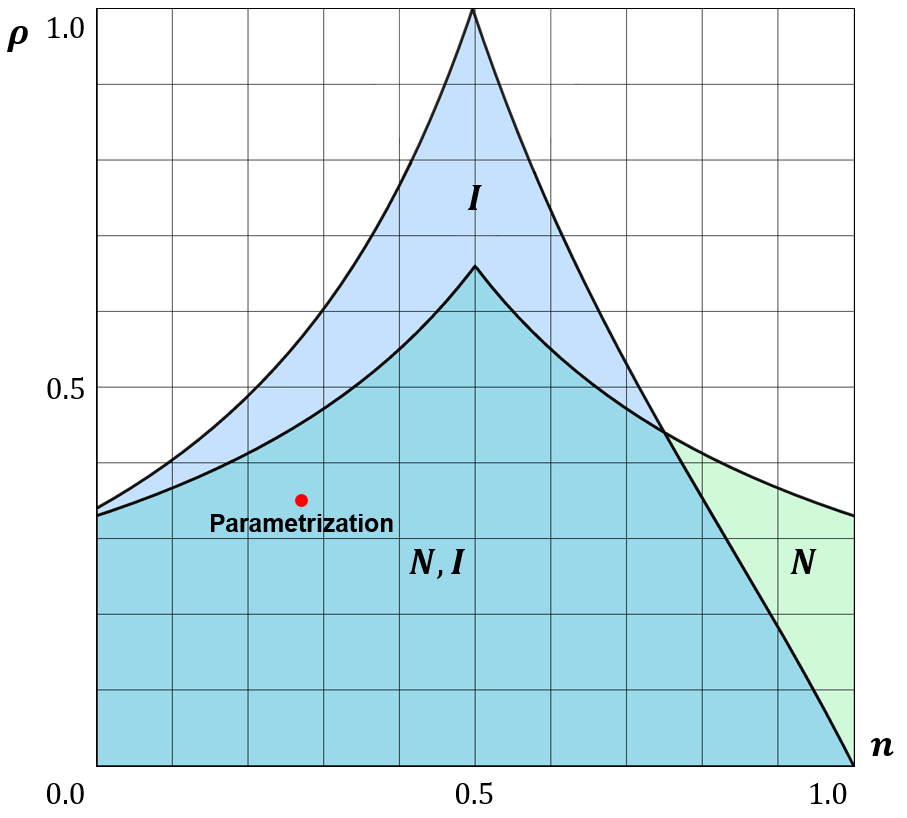
\includegraphics[scale=0.55]{Control-A.PNG}
     \label{fig:im1}

\end{figure}

\begin{figure}
    
    \caption{Typology of equilibria for model with taxes}
    \centering
    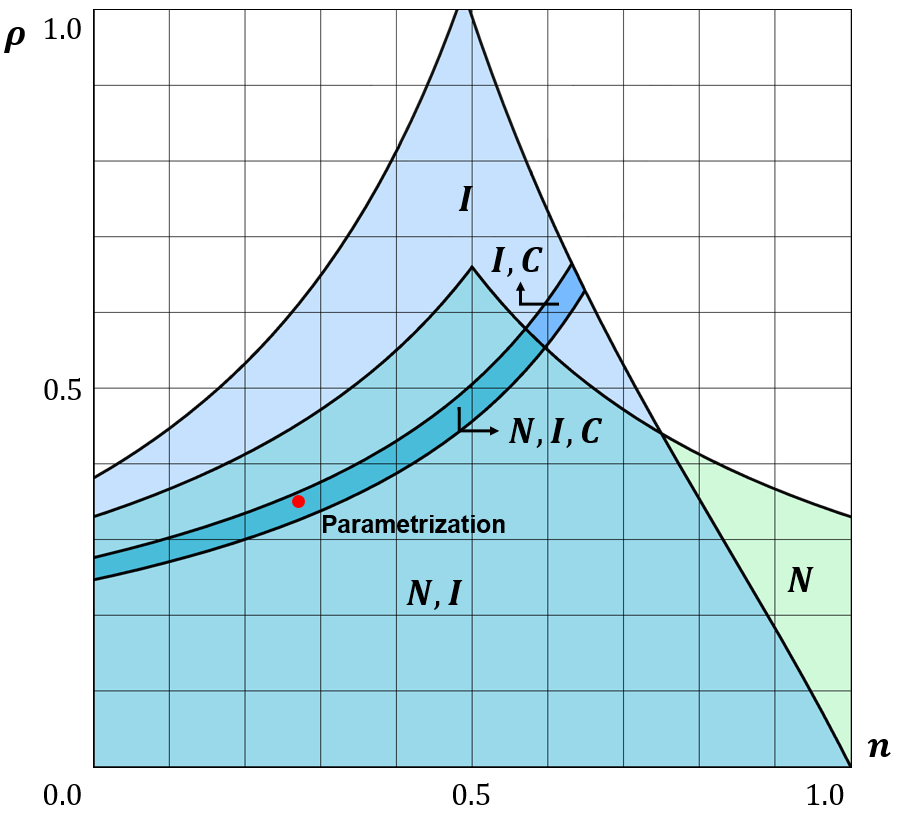
\includegraphics[scale=0.55]{Treatment1-A.PNG}
     \label{fig:im1}

\end{figure}

\begin{figure}
    
    \caption{Typology of equilibria for model with storage costs}
    \centering
    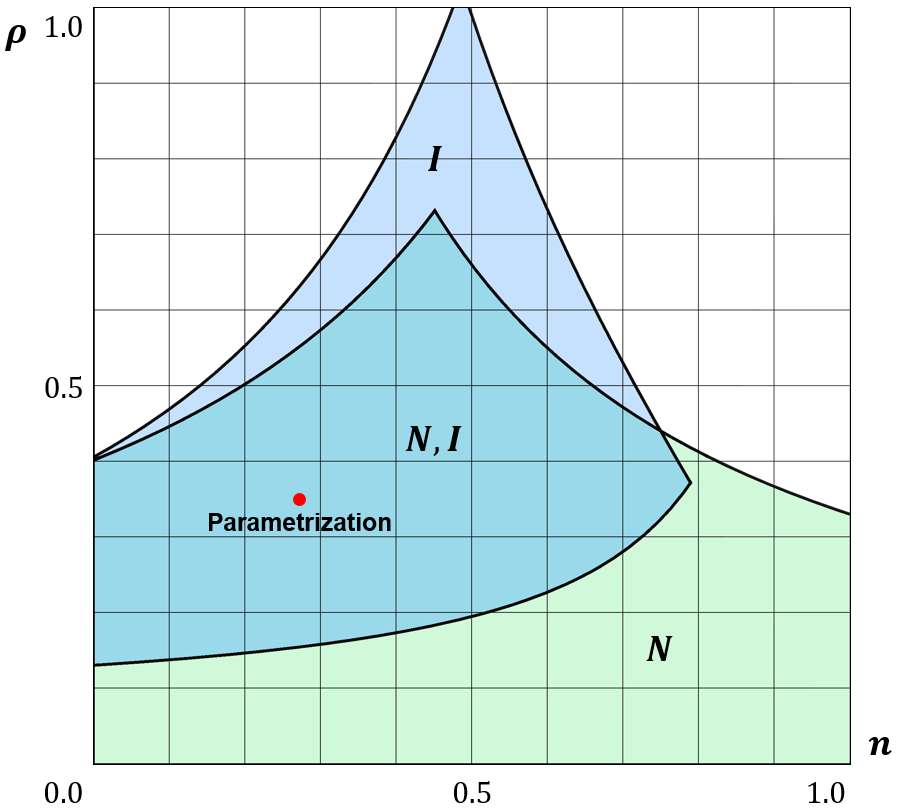
\includegraphics[scale=0.55]{Treatment2-A.PNG}
     \label{fig:im1}

\end{figure}


\section{Experiment Design} 
\label{Experiment}
% \subsection{Experimental Design}
The experimental environment follows closely the model described above, where citizens of two economies repeatedly interact with each other and with citizens of the other economy. 
One of the economies (\textit{Blue}) is set to be the larger economy and the other (\textit{Red}) as a small, open economy whose government implement policies to discourage the domestic use of foreign currency. Since we want to focus on the latter economy, we automated \textit{Blue} citizens, and human participants always operate as citizens of the Red economy.  In particular, we set the size of the \textit{Blue} economy to 20. Meanwhile, groups of eight human participants were assigned to the corresponding \textit{Red} economy. That is, from the perspective of subjects, groups of eight participants are randomly formed and remain for all periods in the experimental session. 
% Here note on discrete / finite population

In each period, individuals participate in the same exchange game described in the theory section. Each agent holds one of three objects: a consumer good, a \textit{Blue} token or a \textit{Red} token. Then, each participant is matched randomly with another agent (observing the partner's origin and object) and needs to decide whether she wants to attempt to exchange objects with partner. Trade attempts occur simultaneously and privately. Once both matched players submit their decisions, these are revealed and the exchange occurs only if there is a mutual willingness to trade objects. As in the model, bartering between sellers (good holders) is not allowed. Same is true for the exchange of tokens. The automated blue agents of the foreign economy always use their optimal trading rule of only accepting blue tokens in exchange for the consumption good and always willing to trade when holding a token. This rule is public information for every participant.

In either country --\textit{Red} or \textit{Blue}-- half of the agents receive their corresponding domestic currency as an initial endowment and the remaining half receive a consumption good. That is, using the model's notation: while $n_b > n_r$, we have $M_B = M_R = 0.5$. We calibrate the integration level so that: (a) there is a higher probability of meeting with another domestic agent for red participants ($\alpha_{rr}=0.75, \alpha_{rb}=0.25$), and (b) there is almost certainty of finding of meeting with another blue agent for blue bots ($\alpha_{bb}=0.9, \alpha_{br}=0.1$).

The interaction is repeated for 50 periods ($T=50$).\footnote{We use a discount factor of $\beta = 0.98$ in calculating our theoretical equilibria. This discount factor was chosen so that, in the analogous model with random stop where probability of continuation equals $\beta$, the average number of periods was 50.} 
Moreover, each human participant starts the first period with an endowment, $W$, of $50$ points, and the consumption utility service, $u$, is 10 points.

There are two additional notes related to departures of the experimental environment from the theoretical model presented above. The first one is related to the fact that we use a finite horizon ($T<\infty$) while in the model time is infinite. On this regard, similar to what is noted in \cite{JiangZhang}, in our environment, there exists monetary equilibria despite the finite horizon. This is in contrast with models where there is a unique monetary equilibrium or those without fiat money, cases which moves toward autarky. 
In these cases, the theoretical prediction is that the economy moves toward autarky. 
% is this sentence correct? j: Yes, with an unique equilibrium, there are incentives to anticipate and avoid trading each round, when you roll the tree, you tend to autarky
Also, we should note that the experimental evidence on monetary economies suggests that money emerges as a medium of exchange in most sequential games with multiple equilibria, but also in those without theoretical monetary equilibrium \citep{RePEc:fip:fedrwp:19-02}. 
% Johar Edita esto: me copie de tu parrafo, pero puse más. In process
% Even though the experiment duration is finite, there is supporting evidence that money emerges as a medium of exchange in sequential games with multiple equilibria. These findings contrast with the cases without fiat money that tend to autarky or the case with an unique equilibrium, which would converge to autarky following backward induction \citep{RePEc:fip:fedrwp:19-02}. johar: listo!

Second, in the model, the population of both countries is modeled as a continuum (with uncountable citizens), while in the experiment, we are naturally forced to work with finite populations in both countries. We chose the appropriate parameters so that the relevant probabilities are compatible with the discreteness of the population. 
Similarly, we chose population sizes that are at least as large as those in \cite{JiangZhang}. They show through simulations that, if the sizes of the economies are sufficiently large, and parameters of the environment are properly chosen, the finite-population model shares relevant equilibria with the infinite population model.

\subsection{Policy Treatments}
Our experiment follows a between-groups design, where each group of eight participants interacted in 50 rounds under a single condition (policy treatment). We implemented the following three policy treatments along with the baseline condition   
\begin{itemize}
\item[] \textbf{Baseline Condition.-} In this control condition, each group of eight human participants form a red country of size eight and interact in 50 rounds of the exchange game described above amongst themselves and with 20 automated blue agents that form the blue economy. The rest of parameters are as given above: $\alpha_{rr}=0.75$, $\alpha_{bb}=0.9$, $W=50$, $u=10$. Storage costs of either token in the red economy are null, $c_r = c_b = 0$. Likewise, taxes for trading with a blue token domestically are $\tau_{r}^{0} = \tau_{r}^{b} = 0$.
% \item In this treatment, the parameterization admits the national and international circulation regime. % make sure we say this hidden sentence later

\item[] \textbf{Treatment 1} \\
In this treatment we maintain the setting of the baseline condition but implement taxes to domestic transactions in foreign currency. In principle, the taxes will be set at $\tau_{S} = \tau_{C} = 1$ point. But the calibration of the actual tax level will be reached when we solve for the equilibria in the extended model presented above. 
% \item In this treatment, the parameterization admits the national, conditional acceptance and international circulation regime.
    
\item[] \textbf{Treatment 2} \\
In this treatment we maintain the setting of the baseline condition but implement asymmetric storage costs of $c_i = 0$ and $c_j = 0.7$. That is, it is more costly to hold foreign currency. In this treatment, the parameterization admits the national and international circulation regime.

\item[] \textbf{Treatment 3} \\
In this treatment we maintain the setting of the baseline condition but implement an information policy about the transactional dollarization. This will show the fraction of exchanges that are made with a foreign currency between locals. In this treatment, the parameterization admits the national and international circulation regime.
\end{itemize}
    %(robot) government who participates in trading withdrawing foreign currency in exchange for a unit of consumption good. 

\end{itemize}

% Equilibrium?
  

\subsection{Metrics and Hypotheses}

The main metric that we study in this paper is the \textbf{acceptance rate of the foreign currency.} At the individual level, this is defined as the binary decision to accept a foreign token in exchange for the consumption good. At the economy level, this metric is defined simply as the percentage of citizens who accept the foreign currency. 

Another important metric associated with efficiency in this environment, is simply the percentage of participants who decide to trade. 

We use the theoretical predictions of the model presented earlier to form the following hypotheses about the experimental results.

\begin{itemize}
\item[] \textbf{Hypothesis I}: The introduction of taxes to domestic transactions in foreign currency, $\tau_S > 0$ and $\tau_C>0$, reduces the acceptance rate of foreign currency. Furthermore, this effect would be based on the trade rejection of foreign currency held by locals. Therefore, we would observe a conditional acceptance regime (\textit{Blue} token accepted for foreign transactions and rejected between domestic agents). 

\item[] \textbf{Hypothesis II}: The introduction of heterogeneous storage costs, $c_j > c_i$ , diminishes the acceptance rate of foreign currency, whether the partner is local or foreigner. Therefore, we should observe  the national currency regime. 

\item[] \textbf{Hypothesis III}: The introduction of information on foreign currency transactions reduces the acceptance rate of foreign currency transactions, as it functions as a coordination mechanism. Hence, we would have a national currency regime.

\item[] \textbf{Hypothesis IV}: The acceptance ratio of the consumption good remains constant throughout the control and treatment sessions. This is a rationality test for the participants, accepting the exchange is a strictly dominant strategy for buyers. 

\item[] \textbf{Hypothesis V}: The acceptance rate of the local currency is higher than the acceptance ratio of the foreign currency, and remains constant through the control sessions and treatment. 


Our results might deal with cooperation issues, given the experimental design. However, there is robust evidence that a lower number of rounds and anonymous random matching reduce the probability of cooperation. On the other hand, public information and perfect monitoring might induce to cooperation, as there are punishment mechanisms available if some agents deviate (in this case the trade rejection). These factors are considered for our analysis, given their importance in the results reported in repeated games \citep{10.1257/jel.20160980}.

\end{itemize}

\subsection{Procedures}

In December 2019, we conducted experimental sessions applying the baseline and the three treatments. In this pilot study, the \textbf{baseline condition} or control groups exhibited two countries with imperfect trade integration, implying a higher probability for encountering a local participant ($\alpha_{ii} = 0.75$) than with a foreign participant ($\alpha_{ij} = 0.25$). 

In the same way, automatized participants of \textit{Blue} group have a higher probability of meeting between themselves ($\alpha_{jj}=0.9$) rather than with a \textit{Red} participant ($\alpha_{jj}=0.1$). In addition, the storage costs were set to zero, $c_i = c_j = 0$. In this setting, the model predicts the equilibrium is characterized by the universal circulation of both currencies. 

We implemented three treatments. In \textbf{Treatment 1}, we implement taxes to domestic transactions in foreign currency. For this parameterization, there are multiple equilibria which could emerge, such as international, national and conditional acceptance regimes. In \textbf{Treatment 2}, we set different storage costs of $c_i = 0$ and $c_j = 0.7$. In this setting, the equilibria is characterized by the national or the international circulation regime. Finally, in \textbf{Treatment 3} we implement an information shock about the transactional dollarization. This will show the fraction of exchanges that are made with a foreign currency between locals.


% \subsection{Implementation}

The experiment was conducted in online sessions with the subject pool from a standard ORSEE server (Greiner, 2015) maintained by the Experimental Economic Laboratory of the Pontifical Catholic University of Peru on December 2019. Upon arrival, each student was assigned a random number between 1 and 8 to participate. 

Our proposed design is \textit{between-group}. That is, participants made decisions in only one of the four conditions described above: the control and the three treatments. Participants knew in advanced that they only will face one treatment. Each of the four blocks (conditions) had 50 periods. The duration of the whole session was one and a half hours. 

Participants received payments based on their performance and they had a participation fee of 5 PEN. The conversion rate was 0.05 soles per point obtained, which was public knowledge. Human subjects earned between 10 and 15 PEN (on average, 13 PEN). The UI software was mainly developed at the LEEPS Lab of the University of California at Santa Cruz using an oTree framework (Chen et al, 2013) and the server was deployed on Heroku servers. 

We follow \cite{JiangZhang} experiment, as they ran 4 sessions for each of their four treatments. In our case, we ran eight sessions, with two groups of 8 participants for each one. Therefore, we had 4 groups for each one of our treatments. 

At the beginning of each session, there was a instructions page. Then, the participants read them and solve incentivized control questions. The experimenters answered for any questions in private via web. 

Each round consisted of a screen presenting individual information and the exchange decision and the results of the round. The screen informed the participants about their own state, as well as the state of its partner and the history of their individual transaction. This included the group to which the players belonged (\textit{Blue} or \textit{Red}), the object carried by each one (\textit{Blue} coin, \textit{Red} coin or consumer good) and their roles in the exchange (buyer or seller). 

There is only one case in which trade exchange was possible: the encounter between a buyer and a seller. If this condition was met, each participant had the option of intending exchange simultaneously. In the case where \textbf{both agents respond positively}, the token and the consumption good are \textbf{exchanged}. Therefore, the consumer consumes the good and produces a new consumption good, while the producer obtains the token, changing roles for the next round.

In any other case, the following message was displayed: \textit{You cannot exchange with your counterpart, since both are buyers (sellers)}. Hence, they did not have any option and passed to the next screen of the game. 

After all the participants in the group had played, they passed to the next round. Subsequently, the exchange was decided and the process continued, successively, until completing the 50 rounds. Finally, they answered a post-interaction survey, oriented to improve future implementations. At the end of the session, we made cash payments following standard procedures of privacy via web transactions. 


\section{Results}

We focus this analysis on the acceptance ratios of the consumer good and the currencies, with a special emphasis on the acceptance rate of the foreign currency (the \textit{\textit{Blue}} economy). This metric presents the different acceptance behavior if the counterpart is a foreigner with the \textit{Blue} token or if she is a local with the object. We present these rates, by control and treatment groups and counterpart type, in Figure 4. 

Figure 4 shows the acceptance rate of the foreign token throughout the four treatments and by different token holder. This ratio is calculated as the number of times that consumers attempted to trade the foreign token for a consumption good over the total number of times in which the exchange was possible. The results show average acceptance rates of 60 percent in the baseline and the transaction history treatment. Both treatments are statistically equivalent. On the other hand, the taxes and storage costs treatments have lower acceptance rate near 40 percent, as they discourage foreign currency circulation at the domestic level.

In fact, if the counterpart is a foreigner, there is a lower acceptance probability for each of the treatments. This might be explained due to the foreign acceptance rule and that all the participants know that foreigners will not accept the local token and, therefore, they would not trade in retribution. Nevertheless, we do not observe a significant difference with the origin of the trading partner. Also, the storage cost treatment is the one with the lowest acceptance probability, due to the penalty applied. 

% Acceptance rate of the foreign token
\begin{figure}
    
    \caption{Foreign token acceptance rate}
    \centering
    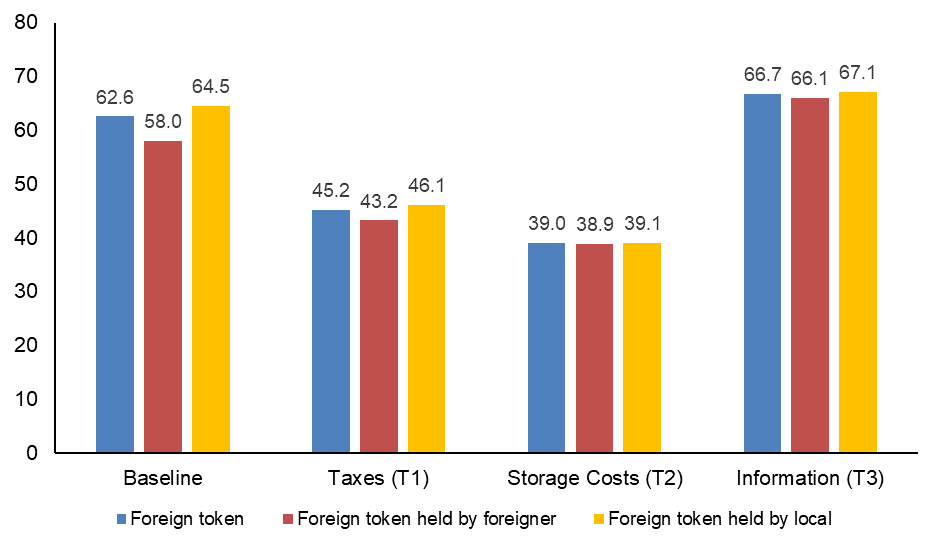
\includegraphics[scale=0.8]{summary.png}
     \label{fig:im1}

\end{figure}

  Foreign currency acceptance rate estimates are presented using the marginal effects of a probit model. We use dummy treatment variables to assess whether these have any effect on the rates of acceptance of the coins. In addition, we include controls referring to the period number and the group effect, which takes into account the effect of learning and cooperation issues within each session. We drop the first 10 rounds to reduce the volatility of the initial learning process. Finally, we cluster the standard errors by group level. Hence, we can control the variance to the possible behavior within each group.


\begin{center}
\begin{tabular}{lccc}
\multicolumn{4}{c}{Table 1: Marginal effects on FC acceptance rates (Probit)} \\ \hline
 & (1) & (2) & (3) \\
Variables  & Full sample & FC held by local & FC held by foreigner \\ \hline
 Taxes [T1]  & -0.167** & -0.169** & -0.205* \\
 & (0.0708) & (0.0806) & (0.110) \\
Storage costs [T2] & -0.204** & -0.289** & -0.191** \\
 & (0.0971) & (0.130) & (0.0901) \\
Information [T3] & 0.0639 & 0.0665 & 0.0134 \\
 & (0.0666) & (0.0915) & (0.0950) \\
 Controls  & \checkmark & \checkmark & \checkmark \\

 N & 759 & 450 & 309 \\ \hline
 
\multicolumn{4}{l}{ Standard errors clustered at the group level in parentheses} \\
\multicolumn{4}{l}{ *** p$<$0.01, ** p$<$0.05, * p$<$0.1} \\
\end{tabular}
\end{center}

Table 1 confirms that taxes and storage costs are the treatments with the major effect in the rejection of foreign token. Specifically, these treatments have significant effects on the acceptance probability of the foreign currency  for all the cases, whether the token holder is local or foreigner. 

Nevertheless, the tax has a lower negative effect if the currency holder is from the \textit{Blue} group, even though there is no tax for this transactions. This happen because, in the case of matching with a foreigner, the participants would anticipate a future negative effect. As there are more chances to meet with a local in future rounds, future local matches would end in rejections if the participant accepts the \textit{Blue} token, given that other locals would prefer to avoid the tax payment. This would be an indirect effect of matching with foreigners in the \textbf{conditional acceptance regime}, as there are asymmetric probabilities against the foreign group. In sum, there are mixed results respect to \textbf{hypothesis I}, as it seems that foreign token is rejected for locals and foreigners, but in different magnitudes, given the asymmetric probabilities for the local group. 

Storage costs maintain its negative effect on the acceptance rate for every counterpart's origin. Furthermore, this treatment has higher marginal effects in all the regressions used. This would confirm the \textbf{hypothesis II}, as storage costs (T2) would reduce the foreign token acceptance and tend to the national currency regime, whether the object is held by a local or a foreigner partner.  

Finally, the information treatment does not have any statistical effect on foreign token probability, rejecting the \textbf{hypothesis III}. Results are not statistically nor descriptive different from the baseline condition. The null effect reflects that information differences on group behavior do not have major effects on individual behavior. This behavior might be explained in the random encounters participants had in little groups, which deters coordination possibilities \citep{10.1257/jel.20160980}.

\begin{center}
    \begin{tabular}{lcc}
\multicolumn{3}{c}{Table 2: Marginal effects on HC and good acceptance rates (Probit)} \\ \hline
 & (1) & (2) \\
Variables & Home token & Consumption good \\ \hline
 Taxes [T1] & 0.156*** & -0.0519 \\
 & (0.0410) & (0.0381) \\
Storage costs [T2] & 0.190*** & -0.0784 \\
 & (0.0388) & (0.0626) \\
Information [T3] & 0.0575 & -0.0304 \\
 & (0.0409) & (0.0401) \\
 Controls  & \checkmark & \checkmark \\
 N & 697 & 1,523 \\ \hline
 
\multicolumn{3}{l}{ Standard errors clustered at the group level in parentheses} \\
\multicolumn{3}{l}{ *** p$<$0.01, ** p$<$0.05, * p$<$0.1} \\
\end{tabular}
\end{center}

Furthermore, we analyze additional measures to prove hypothesis on participants' behavior. Results on consumption good show that none of the treatment nor the controls have impact on the acceptance probability. These findings coincide with the \textbf{fourth hypothesis} that the consumption good should always be accepted (it is rational -in fact a dominant strategy- that all buyers choose to accept the consumption good), regardless the treatment.


Finally, the treatment effects on home currency acceptance have heterogeneous results that reject the \textbf{fifth hypothesis}, because the first two treatments have significant and positive effects on accepting the local token. Both treatments diminish the foreign acceptance and enhance the local currency circulation, while the information policy does not have any statistical effect.  




\section{Discussion} 

Our main results are that, in line with theoretical predictions, a policy that increases the storage costs of money or one that taxes specific transactions can influence the currency acceptance decisions. 

\begin{itemize}
    \item Storage costs have negative and significant effects on the foreign currency acceptance probability for all the possible partner's origin
    \item Transaction taxes diminish the foreign token acceptance for both cases but in a different magnitude: there is a strongest rejection when meeting a local than a foreigner, that might serve as a basis for a conditional acceptance regime
    \item Information on foreign currency transactions does not seem to have effect on the acceptance probability, as there are no incentives to coordinate on a regime different that the baseline.
    \item Home currency acceptance is enhanced by the taxes and the storage costs treatments, contrary to the belief that they would stay constant across the treatments.
    \item Consumption good acceptance rate remains constant across rounds and sessions, as it is a dominant strategy and could be used as a verification test.
\end{itemize}

% However, we also document some interesting discrepancies between the theoretical and experimental results on the circulation of foreign currency with partial integration.

Hence, we propose to extend the experimental design and the theoretical framework to focus in the circulation of foreign currency among agents of the same economy. This happens, for example, in Latin American economies and it is called \textit{transactional dollarization}. Interestingly, this type of dollarization has not been as researched as \textit{financial dollarization}. \citep{RePEc:imf:imfwpa:05/187, armas16}  % cite the hell out of financial dollarization 

Taking our prediction to the empiricism, there are different results for monetary outcomes if economies decide to tax foreign transactions or imposing a holding costs. Empirical results show that holding costs might be seen as reserves requirements or macroprudential policies taken by the Central Banks. On the other hand, transactional taxes are decided by the Finance Ministry and the International Relations Ministry, as it affects international trade. Evidence on emerging economies show that implementation would be easier in the case of macroprudential policies for independent Central Banks. Meanwhile, transaction taxes were proposed in Europe with the Currency Transaction Tax in early 2000s, but it was not applied until Argentinian tax on foreign currency transactions, mainly in dollars. 

Additionally, we aim to complement the theoretical and experimental framework to include effects on the welfare of the economy. In the experiment documented above, it is shown that the introduction of differentiated costs and transaction taxes incentive a system of local circulation. However, the implications on welfare are not well defined, and, we will include that aspect in future versions. Specifically, we need to develop a framework which would redistribute the taxes in a welfare-improving method. Otherwise, both treatments would have the same dynamic.

Future extensions of this article would change the experimental design to include a higher number of rounds and increase the size of the foreign economy. With these considerations, we may solve the possible problems of coordination and the difficulties of getting a fiat money currency equilibrium in a finite game \citep{10.1257/jel.20160980, RePEc:fip:fedrwp:19-02}. Finally, we should complement the information treatment by eliciting belief priors and evaluate the findings with the experimental results.


% Finally,  the experiment with the between-group design should be considered for prevent the same session dynamics from inducing the expected results. 

%%%%%%%%%%%%%%%%%%%%%%%%%%%

\bibliographystyle{apalike}
\bibliography{References.bib}

%%%%%%%%%%%%%%%%%%%%%%%%%%%

\newpage
\appendix

\begin{center}
\huge{\textbf{Appendix}}
\end{center}

\section{Solutions to the Analytical Model}

 Policies for de-dollarization \\
General set-up follows \citep{MKM}\\ 
 Modifications made on the lab: \\
 A. Matching technology\\ 

 \begin{table}[tbh]
\begin{tabular}{lll}
 & Home & Foreign \\
Home & 1 - $\beta( 1 - n )$ & $\beta ( 1 - n )$ \\
Foreign & $\beta n$ &  $1- \beta n$
\end{tabular}
\end{table}

$\beta \in (0,1)\\  
 n = \frac { N_H } { N_H + N_F } $
\\

\textbf{Control group}\\
\textbf{Equilibrium F} (foreign currency is the international currency)\\

We need to state the condition of holding a local and a foreign currency for the local economy:\\

$m _ { h } = m , m ^ { * }_h = 0$\\
We need $m _ { f } , m _ { f } ^ { * } > 0$ such that $n m_ { f } + ( 1 - n ) m _ { f } ^ { * } = ( 1 - n ) m ^ { * }$\\

Stationarity requires that $\frac{m _ { f }}{1-m-m_f} = \frac{m^* _ { f }}{1-m _ { f } ^ { * }}  $\\

$m _ { f } - m _ { f } m _ { f } ^ { * } = m _ { f } ^ { * } -m m _ { f } ^ { * } - m _ { f } m _ { f } ^ { * }$\\

$m _ { f }= (1- m) m _ { f } ^ { * } $\\

Combining the market-clearing condition is the result found above:

$n(1-m)m _ { f }^* +( 1 - n)   m _ { f } ^ { * } =(1-n)m^*$\\


$m _ { f } = \frac { 1 - n } { 1 - m _ { n } } m^*$\\

$m_ { f } = \frac { ( 1 - m ) ( 1 - n ) } { 1 - m n }m^* $\\

Then, we determine the value functions for the equilibrium in the case an agent has a consumption good ($V_C$), a local currency ($V_h$) and a foreign currency ($V_f$). :\\

$(1+\delta)V_C=\alpha _ { h h }(m V _ { h } +m_fV_f+(1-m-m_f)V_C)+ \alpha_{hf}(m_f^*V_f+(1-m_f^*)V_C)           $

$V _ { C } = \frac { \alpha _ { h h } m V _ { h } + \left( \alpha _ { h h } m _ { f } + \alpha _ { h f } m _ { f } ^ { * } \right) V _ { f } } { 1 + \delta - \alpha_{h h} \left( 1 - m - m _ { f } \right) - \alpha {h f } \left( 1 - m _ { f }^* \right) }$\\


$( 1 + \delta ) V_ h = \alpha_{hh} \left( m V _ { h } + m _ { f } V_h + \left( 1 - m - m _ { f } \right) ( u + V_C ) \right) + \alpha _ { hf } \left( m _ { f }^*  V _ { h } + \left( 1 - m _ { f } ^ { * } \right) V _ { h } \right) $\\



$V _ { h } = \frac { \alpha  _ { hh } \left( 1 - m - m _ { f } \right) \left( u + V _ { c } \right) } { 1 + \delta - \alpha_{h h} \left( m + m _ { f } \right) - \alpha  _ { hf } }$ \\





$( 1 + \delta ) V _ { f } = \alpha _ { h h } \left( m V _ { f } + m _ { f } V _ { f } + \left( 1 - m - m _ { f } \right) \left( u _ { 1 } V _ { C } \right) \right) + \delta_{hf} \left( m _ { f }^* V _ { f } + \left( 1 - m _ { f }^* \right) \left( u + V _ { C } \right) \right)$ \\



$V _ { f } = \frac { \left( \alpha _ { h h } \left( 1 -m- m _ { f } \right) + \alpha _ { h f } \left( 1 - m _ { f } ^*\right) \right) \left( u + V _ { C } \right) } { 1 + \delta - \alpha {h h} \left( m + m _ { f } \right) - \alpha {h f } m _ { f }^* }$\\

Unambiguously, $V_{f} > V _ { h }$ (check expressions in flow terms)\\

$\delta V_C  = \alpha_{hh} m \left( V _ { h }- V _ { C } \right) + \left( \alpha  _ {h h } m _ { f } + \alpha  _ { hf } m _ { f }^* \right) \left( V _ { f } - V _ { C } \right)$\\

$V _ { C } = \frac { \alpha _ { h h } m V _ { h } + \left( \alpha _ { h h } m _ { f } + \alpha_{hf} + m _ { f } ^ { * } \right) V _ { f } } { \delta + \alpha_{h h} m + \alpha_ {h h} m _ { f } + \alpha_h + m _ { f } ^* }$\\

$\delta V _ { h } = \alpha_{hh} \left( 1 - m - m _ { f } \right) \left( u + V _ { C } - V _ { h } \right)$\\

$V h = \frac { \alpha _ { h h } \left( 1 - m - m _ { f } \right) } { \delta + \alpha_{hh} \left( 1 - m - m _ { f } \right) } \left( u + V _ { c } \right)$\\

$\delta V _ { f } = \left( \alpha _ { hh } \left( 1 - m - m _ { f } \right) + \alpha _ { hf } \left(1 - m _ { f }^* \right) \right) \left( u + V _ { C } - V _ { f } \right)$\\

$V _ { f } = \frac { \left( \alpha _{h h} \left( 1 - m - m _ { f } \right) + \alpha _ { hf}  \left(1 - m _ { f }^* \right)  \right) \left( u + V _ { C } \right) } { \delta + \alpha _ { h h } \left( 1 - m - m _ { f } \right) + \alpha _{hf}  \left( 1 - m _ { f }^* \right) }$\\

Unambiguously, $V _ { f } > V _ { h }$\\

$u + V _ { C } > V_h$\\

$u+V_C> V_f$\\

We must verify the following condition: $V _ { h } > V _ { C }$, which means that the seller would accept to give their commodity good instead of a local currency. Incentive compatibility constraint more binding than $V_f>V_C$\\


Also, we need to define the conditions for the equilibrium $F$ in the foreign economy. \\

\textbf{Foreign economy} \\

$ \delta V _ { C  }^ { * }  = \left( \alpha _ { fh }  m _ { f } + \alpha _ { f f } m _ { f } ^* } \right) \left( V _ { f } ^ { * } - V _ { C } ^ { * } \right) $\\

$V _{C}^* = \frac{\left(\alpha _{fh}m_{f} + \alpha_{ff} m_{f}^* \right) V _ { f } ^ * } { \delta + \alpha _ { fh }  m _ { f } + \alpha _ { ff } + m _ { f } ^ { * } }$ \\ 

$V _ { C } ^ { * } = \frac { \alpha _ { ff } m ^ { * } v _ { f ^ { * } } } { \delta + \alpha_{ f f} m ^ { * } }$\\


$ \delta V _ { h  }^ { * }   = \alpha _ { f h } \left( 1 - m - m _ { f } \right) \left( u + V _ { C } ^ { * } - V _ { h } ^ { * } \right)   \\ $

$ V _ { h  }^ { * }   = \frac{\alpha _ { f h } \left( 1 - m - m _ { f } \right) \left( u + V _ { C } ^ { * }\right) }{\delta + \alpha _ { fh } \left( 1 -m- m _ { f } \right) }   \\ $

$V _ { h } ^ { * } = \frac { \alpha _ { f h } ( 1 - m ) \left( u + V _ { c } ^ { * } \right) } { \delta + \alpha_{f h} ( 1 - m ) }$ \\

$ \delta V _ { f } ^ { * }  = \left(\alpha _ { f h } \left( 1 - m - m _ { f } \right) + \alpha_ { ff } \left( 1 - m _ { f } ^ { * } \right) \right) \left( u + V _ { C  }^ { * }-V_f^* \right)   $\\

$ V _ { f } ^ { * }  = \frac {\left(\alpha _ { f h } \left( 1 - m - m _ { f } \right) + \alpha_ { ff } \left( 1 - m _ { f } ^ { * } \right) \right) \left( u + V _ { C  }^ { * } \right) } { \delta+ \alpha _ { f h } \left( 1 - m - m _ { f } \right) + \alpha _{ff} \left( 1 - m _ { f }^ { * }  \right) }  $\\


$ V _ { f  }^ { * } = \frac {  \alpha _ { ff } \left( 1  - m^* _ { f } \right) \left( u + V _ { C } ^ { * } \right) } { \delta + \alpha _ { f f } \left( 1  - m ^* \right) } $\\

Unambiguously,\\

 $u + V_C ^ { * } > V_h ^ { * }$ \\
 
 $u + V_C ^ { * } > V _ { f } ^ { * }$ \\ 
 
 $V _ { f } ^ { * } > V_h ^ { * }$ \\ 
 
 $V _ { C } ^ { * } < V _ { f } ^ { * } $\\


$u + V _ { C } ^* > V_ { h }^ { * }$\\

$u + V _ { f  }^ { * } > V _ { f }^ { * }$\\

$V _ { f  } ^{ * } > V _ { C  }^ { * }$\\

We must verify the following condition: $V _ { C } ^ { * } \geq V_ { h }^ { * }$ \\

This condition must also hold when $m_f=0$ (autarky)\\

Open question: Can we find adequate parameters such that welfare is greater under autarky?\\

\textbf{Treatment 1:} Taxes on domestic transactions made with foreign currency\\

We introduce the taxes on the value functions and evaluate its impact on the stationarity conditions. With this results, we obtain threshold values for both equilibria in function of the parameters and the matching probabilities: \\

$\delta V _ { c } = \alpha _ { h h } m \left( V _ { h } - V _ { C } \right) + \alpha_{h h} m _ { f } \left( V _ { f } - \tau ^ { c } - V _ { C } \right) + \alpha _ { h f } m _ { f } ^* \left( V _ { f } - V _ { C } \right)$\\

$V _ { C } = \frac { \alpha_{h h }m V_h + \left( \alpha _{h H} m _ { f } + \alpha  _ { hf } m _ { f }^* \right) V _ { f } - \alpha _{h h} m _ { f } \tau^c } { \delta +\alpha_{hh}m+\alpha_{hh}m_f+\alpha_{hf}_m_f^*}$\\

$\delta V _ { h } = \alpha _{ hh } \left( 1 - m - m _ { f } \right) \left( u + V _ { c } - V_ h \right)$\\

$V_h = \frac { \alpha_{h h} \left( 1 - m - m _ { f } \right) ( u + V_C ) } { \delta + \alpha_{ h h} ( 1 - m - m_f ) }$\\

$ \delta V _ { f }  = \alpha _ { h h } \left( 1 - m - m _ { f } \right) \left( u + V _ { C } - \tau ^ { f } - V _ { f } \right) + \alpha _ { hf } \left( 1 - m _ { f } ^ { * } \right) \left( u + V _ { C } - V _ { f } \right)$ \\


$V _ { f } = \frac { \left( \alpha_{h h} \left( 1 - m - m _ { f } \right) + \alpha_{hf} ( 1 - m_f^* ) \right) ( u + V_C ) - \alpha_{h h} \left( 1 - m - m _ { f } \right) \tau ^ { f } } { \delta + \alpha_{h h} ( 1 - m - m_f ) + \alpha_ { hf } ( 1 - m_f^* ) } $\\

Unambiguously,\\

$u+ V_C > V_h$ \\

$u+V_C > V _ { f }$\\

\textbf{Equilibrium F}:\\

\begin{enumerate}

    \item $V_f > V_h$ (no currency exchange)
    
    \item $V _ { h } > V _ { C }$
    
    \item $V_f > V _ { C }$
    
\end{enumerate}


We must verify 1, 2 and 3. (1, 2 are sufficient)

\\

\textbf{Equilibrium A}\\

$ m _ { h } = m , m _ { f } = 0 , m _ { h } ^ { * } = 0 , m _ { f } ^ { * } = m ^ { * }$ \\


  $V _ { C } = \frac { \alpha _ { hh } m V _ { h } } { \delta + \alpha_{hh  } m} \\ $
  
  $V _ { h } = \frac { \alpha_{hh} ( 1 - m ) \left( u + V _ { C } \right) } { \delta + \alpha_ { hh } ( 1 - m ) } } \\ $
  
   $V _ { f } = \frac { \alpha_{hf} ( 1 - m ) \left( u + V _ { C } \right) } { \delta + \alpha _ { hf } \left( 1 - m ^ { * } \right) } } $\\
   
Unambiguously, $u + V _ { C } > V _ { h } , \quad V _ { C } < V _ { h }$\\

$u + v _ { C } > v _ { f }$\\

We must verify that $V _ { C } \geq V _ { f }$. (Incentive compatibility constraint)\\



\textbf{Treatment 2}: Storage cost on foreign currency

Equivalently, we must state the impact of a storage cost on foreign currency in the value functions of each option and verify the conditions previously found\\

$$
 \delta V _ { C } = \alpha_ { hh } m \left( V _ { h } - V _ { C } \right) + \alpha  _ { hh } m _ { f } \left( V _ { f } - V _ { C } \right) + \alpha_{ hf }  m _ { f } ^ { * } \left( V _ { f } - V _ { c } \right) \\
 
 $V_C = \frac { \alpha _ { h h } m \left( V _ { h } - V _ { C } \right) + \left( \alpha _ { hh } m _ { f } + \alpha _ { hf} m _ { f } ^ { * } \right) \left( V _ { f } - V _ { C } \right) } { \delta + \alpha _{hh} m + \alpha _ { h h } m _ { f } + \alpha _ { h f } m _ { f }^* } \\ $
 
 $\delta V_h =  \alpha _{h h}\left( 1 - m - m _ { f } \right) \left( u + V _ { C } - V_h \right) \\$
 
 $V_ h =  \frac { \alpha_{h h}\left( 1 - m - m _ { f } \right) \left( u + V _ { C } \right) } { \delta + \alpha_{hh}  ( 1 - m - m_f ) }$ \\ 
 
$\delta V _ { f } = \left( \alpha _ { h h } \left( 1 - m - m _ { f } \right) +\alpha  _ { hf } \left( 1 - m _ { f } ^ { * } \right) \right) \left( u + V _ { C } - V _ { f } \right)\\

& - \left( 1 - \alpha _ { hh } \left( 1 - m - m _ { f } \right) - \alpha_ { hf }  \left( 1 - m _ { f } ^ { * } \right) \right) \tau$\\


$V_f= \frac { \left( \alpha_{hh}\left(1-m-m_{f}\right) +\alpha_ {hf} \left(1-m_{f} ^* \right) \right)\left(u+V_{C} \right) - \left(1-\alpha_{hh} \left(1-m-m_{f} \right) - \alpha_{ hf}\left(1-m_{f} ^ { * } \right) \right) \tau } {\delta + \alpha _ { hh } \left( 1 - m - m _ { f } \right) + \alpha _ { hf } \left( 1 - m _ { f } ^* \right) }$\\

$V_f= \frac { \left( \alpha_{hh}\left(1-m-m_{f}\right) +\alpha_ {hf} \left(1-m_{f} ^* \right) \right)\left(u+V_{C} \right) - \left(\alpha_{hh}m +\alpga_{hh}m_f+ \alpha_{ hf}\left(m_{f} ^ { * } \right) \right) \tau } {\delta + \alpha _ { hh } \left( 1 - m - m _ { f } \right) + \alpha _ { hf } \left( 1 - m _ { f } ^* \right) }$\\

Once again, we must verify 1, 2 and 3 \\

\textbf{Welfare analysis}\\

Furthermore, we define the welfare of both treatments in function of the fundamentals and the taxes imposed. Then, we need to find a tax level that give the same welfare for both policies. \\

\textbf{Treatment 1}\\

$
 W^1 gov  \propto \frac { \alpha _{hh} ( 1 - m - m_f ) m_f \tau ^ { c } } { \delta + \alpha_{hh} m + \alpha _ { hf } \left( m _ { f } + m _ { f } ^ { * } \right) } + \frac { \alpha_{hh} \left( 1 - m - m _ { f } \right) m_f+ \tau ^ { f } } { \delta + \alpha_{h h} ( 1 - m - m_f ) + \alpha_ { hf } \left( 1 - m _ { f } ^ { * } \right) }\\
$


\textbf{Treatment 2}\\

 $ W^2 gov \propto \frac { \left( \alpha _ { h h } m + \alpha _ { h h } m _ { f } + \alpha _ { h f } \left( 1 - m _ { f } ^ { * } \right) m _ {f} \tau \right} { \delta + \alpha  _ { hh } \left( 1 - m - m _ { f } \right) + \alpha _ { h f } \left( 1 - m _ { f } ^ { * } \right) }$\\
 
We must find $\tau ^ { c } , \tau ^ { f }$ and $\tau$ such that $W ^ { 1 }_{gov}$ $= W _ { \text {gov } } ^ { 2 }$\\


\textbf{Multiple equilibria (control group)}\\

Propositions from \cite{MKM}\\

Finally, we need to define the equilibria conditions based on the transition matrix, $P_ij$ and the model fundamentals:\\

\textbf{Equilibrium A}: $V_C\geq V_f$ iff $ P _ { f C } \left( \delta + P _ { C h } + P _ { h C } + P _ { h f } \right) + P _ { f h } P  _ { hC } \leq P_{Ch}P_{hC}$\\

$\beta ( 1 - n ) \left( 1 - m ^ { * } \right) ( \delta + 1 - \beta ( 1 - n ) ) \leq ( 1 - \beta ( 1 - n ) ) ^ { 2 } m ( 1 - m )$\\



$P _ { f C } = \alpha _ { \text {hf } } \left( 1 - m ^ { * } \right)$\\

$P _ { C h } = \alpha_{hh} m$\\

$P_hC = \alpha_{hh} ( 1 - m )$\\

$P_{hf}= 0$\\

$P _ { f h } = 0$\\

$P _ { C f } = 0$\\

$\alpha _ { h h } = 1 -\beta ( 1 - n )$\\

$\alpha _ { h f } = \beta ( 1 - n )$\\


Analogously for the foreign economy, \\

$V _ { C } ^ { * } \geq V _ { h } ^ { * }$ iff $ P_{ hc }^ { * } \left( \delta + P_ { Cf } ^ { * } + P _ { f C } ^ { * } + P _ { fh } ^ { * } \right) + P  _ { hf } ^ { * } P _ { f C } ^ { * } \leq P _ { C f } ^ { * } P _ { f C }^*$\\

$\beta n ( 1 - m ) ( \delta + 1 - \beta n ) \leq ( 1 - \beta n ) ^ { 2 } m ^ { * } \left( 1 - m ^ { * } \right)$\\

$P _ { fC }^*  = \alpha_ { f f } ( 1 - m^* )$\\

$P_{Ch}^* = 0$\\

$P_{hC}^* = \alpha _ { fh } ( 1 - m )$\\

$P _ { h f } ^f= P _ { f h}^* = 0$\\

$P_{Cf}^* = \alpha _ { f f } m^*$\\


\textbf{Equilibrium F}: 

$ V_h > V_C$ iff $P_{ hC } \left( \delta + P_{C f} + P _ { f C } + P _ { f h } \right) + P _ { hf } P _ { f c } > P _ { C f } P_{fC}$\\

$P _ { h C } = \alpha _ { h h } \left( 1 - m - m _ { f } \right)$\\

$P _ { C f } = \alpha _ { h h }m_f+\alpha_{hf}m_f^*$\\

$P _ { f C } = \alpha_{hh} \left( 1 - m - m _ { f } \right) + \alpha  _ { hf } \left( 1 - m _ { f }^* \right)$\\

$ P _ { fh }  = P _ { h f } = 0$ { (note that $P_{hC } < P _ { f C }$ implies that $V _ { h } < V _ { f })$ \\

$\alpha_{hh}\left( 1 - m - m _ { f } \right) \left( \delta + \alpha _{h h} m _ { f } + \alpha  _ { hf } m _ { f } ^ { * } + \alpha_{hh} \left( 1 - m - m _ { f } \right) - \alpha _ { hf } ( 1 - m _ { f } ^ { * }) \right) > \\

& \left( \alpha _{h h} m _ { f }+\alpha  _ { hf } m _ { f } ^ { * }\right)\left(\alpha_{hh}(1-m-m_f)+\alpha_{hf}(1-m_f^*)\right)$\\

$ \alpha _ { hh } \left( 1 - m - m _ { f } \right) \left( \delta + \alpha _{hh} ( 1 - m ) + \alpha  _ { hf } \right)> \left(\alpha _ { hh } m _ { f }+\alpha _ { hf } m _ { f  ^ { * } \right) \left( \alpha_{hh} ( 1 - m - m _ { f } ) \\

& + \alpha _ { hf }  ( 1 - m _ { f } ^ { * } ) \right) \right)$\\

$ \alpha _ { hh } \left( 1 - m - m _ { f } \right) \left( \delta + \alpha _{hh} ( 1 - m ) + \alpha  _ { hf } \right)>(\alpha _ { hh } (1-m)+\alpha _ { hf }) m _ { f}  ^ { * }   ( 1 - m _ { f } ^ { * } )  ( \alpha_{hh} ( 1 - m ) + \alpha _ { hf } )$\\

$ \alpha _ { hh } \left( 1 - m - m _ { f } \right) \left( \delta + \alpha _{hh} ( 1 - m ) + \alpha  _ { hf } \right)>(\alpha _ { hh } (1-m)+\alpha _ { hf })^2 m _ { f}  ^ { * }   ( 1 - m _ { f } ^ { * } )  $\\

$ \alpha _ { hh } \left( 1 - m  \right) \left( \delta + \alpha _{hh} ( 1 - m ) + \alpha  _ { hf } \right)>(\alpha _ { hh } (1-m)+\alpha _ { hf })^2 m _ { f}  ^ { * }     $\\

Analogously for the foreign economy, $V _ { C } ^ { * } \geq V _ { h } ^ { * }$\\

$P _ { f C } ^ { * }= \alpha _ { f f } \left( 1 - m _ { f } ^ { * } \right) + \alpha _ { f h } \left( 1 - m - m _ { f } \right)$ \\

$P _ { C h  } ^ { * }= 0$\\

$P _{h C} ^ { * } = \alpha _ { f h } \left( 1 - m - m _ { f } \right)$ \\

$ P_{ hf }  ^ { * } = P _ { f h } ^ { * } = 0$\\

$P _ { C f } ^ { * } = \alpha _ { f f } m _ { f } ^ { * } + \alpha _ { f h } m _ { f }$\\

$\alpha_{fh}(1-m- m_f)( \delta + \alpha_{ff} m_f^*+\alpha_{fh}m_f+\alpha_{ff}(1- m_f^*)+\alpha _ { fh }(1-m_f)) \leq (\alpha_{ff}m_f^*+\alpha_{fh}m_f)(\alpha_{ff}(1-m_f^*)+\alpha_{fh}(1-m-m_f))$\\

$ \alpha _ { fh }  ( 1 - m )  ( 1 - m^*_f )( \delta + \alpha_{ff}+ \alpha_{fh}(1-m)) \leq (\alpha _ { ff }+ \alpha _ { fh } ( 1 - m )) m _ { f }^* ( 1 - m_f ^*)(\alpha_{ff}+\alpha_{fh}(1-m))$\\

$ \alpha _ { fh }  ( 1 - m )  ( \delta + \alpha_{ff}+ \alpha_{fh}(1-m)) \leq (\alpha _ { ff }+ \alpha _ { fh } ( 1 - m ))^2  m_f^*$\\

$\alpha_{hh} ( 1 - m ) ( \delta + \alpha_{hh} (1-m)+ \alpha_{hf} ) ( 1 - m n ) > ( \alpha _{hh} ( 1 - m ) + \alpha_{hf} ) ^ { 2 } ( 1 - n ) m^*$\\

$\alpha _ {fh } ( 1 - m ) ( \delta + \alpha_{ff} + \alpha_{fh}  ( 1 - m ) ) ( 1 - m n ) \leq \left( \alpha _ { ff } + \alpha_{fh}  ( 1 - m ) \right) ^ { 2 } ( 1 - n ) m^*$\\

Replacing matching probabilities:\\

$( 1 - \beta ( 1 - n ) ) ( 1 - m ) ( \delta + ( 1 - \beta ( 1 - n ) ) ( 1 - m ) + \beta ( 1 - n ) ) ( 1 - m n ) > ( ( 1 - \beta ( 1 - n ) ) ( 1 - m ) + \beta ( 1 - n ) ) ^ { 2 } ( 1 - n ) m ^ { *}$\\

$\beta n ( 1 - m ) ( \delta + ( 1 - \beta n ) + \beta n ( 1 - m ) ) ( 1 - m n ) \leq ( ( 1 - \beta n ) + \beta n ( 1 - m ) ) ^ { 2 } ( 1 - n ) m ^ { * }$


\newpage

\subfile{letter.tex}




\section{Instructions for Participants}

(Translated from Spanish)

Welcome. Thank you for participating in today's session. Read these instructions carefully; your decisions
and those of the other participants of the experiment will determine your payment. This payment will be proportional to the points that you accumulate throughout the experiment. Upon completion, the accumulated points will be transformed into soles (S /) at 1 point conversion rate = S / 0.05. Additionally, you will be paid S / 4.00 just for participating.

\textbf{ Rounds and Groups }
The central block of this session consists of 50 rounds of the same type of interaction. At the start of the first round, random groups will be formed. Each group will have 8 participants. The groups are fixed, which means that throughout the session you will stay in the same group. Your group will be called a \textit{Red} group. The people of your group
will interact with each other and with agents of the \textit{Blue} group, who are represented by the computer (they are bots). In the \textit{Blue} group there are 20 agents.
 
\textbf{ Initial endowments }
Each participant in your group starts the first round with a 50-point endowment and one of two objects: one \textit{Red} token or a consumer good. Half of the Red group members receive a \textit{Red} token, and the remaining half will receive a consumer good. The assigned object is randomly assigned. The situation is analogous to the \textit{Blue} group, where 10 agents receive randomly
a \textit{Blue} token and 10 receive a consumer good. The quantity of each object remains fixed throughout all rounds.
 
\textbf{ Random couples in each round }
At the beginning of the round, each member of the \textit{Red} group is randomly matched with someone from their group or from the \textit{Blue} group. The probability of pairing with someone in the \textit{Red} group is 75\% and with someone in the \textit{Blue} group is 25\%.
 
\textbf{ Exchange Decision }
In each round, every participant is informed of their own object, the group of his partner and the object she has.
Some meetings have trade possibility and others do not. There is only exchange possibility if one has one token and the other has a consumption good. On the contrary, if both people have consumption goods, there is no exchange possibility (no barter). If the two have tokens, they cannot exchange them either. In the case of being possible to exchange, both agents must decide privately whether they want to exchange or not. Only if both agents respond positively, the token and the consumption good are exchanged. \textit{Blue} group agents are automated (they are bots) and are always willing to exchange but never accept \textit{Red} tokens. The object with which you end a round is the same with which you start the next.
 


\textbf{ Payments }
All participants start with 50 points. 

In each round, receiving a token grants 0 points, regardless of whether it is \textit{Red} or \textit{Blue}.
In contrast, receiving a consumption good from another participant gives you 10 points when you receive it.
That is, the consumption good generates points only if it is obtained as a result of an exchange, regardless of which group it comes from.
If you maintain the same consumption good for more than one period, you do not receive additional points. 


\textbf{For the Tax treatment}: 
Using \textit{Blue} tokens between agents of the \textit{Red} group is taxed. 
If you receive a \textit{Blue} token from another participant in the \textit{Red} group, you will pay a 1 point tax.
Similarly, if you exchange a \textit{Blue} token for a consumption good with another participant of the \textit{Red} group, you will pay a 1 point tax.


\textbf{For the Store cost treatment}: 
If you keep a token for more than one period, you will pay a storage cost.
If you keep a \textit{Red} token, you'll pay 0 points.
If you keep a \textit{Blue} token, you will pay 0.7 points.


During all interaction rounds, you will have on your screen the information referred to the previous rounds.

\textbf{For the Information treatment}
In particular,  the acceptance rate of the \textit{Blue} token among people on the red team will be displayed. 


The payment of the session is the accumulated points of the 50 rounds of interaction.



 Bienvenido(a). Gracias por participar en la sesión de hoy. Lee con cuidado estas instrucciones; tus decisiones y las de los demás participantes del experimento determinarán tu pago. Dicho pago será proporcional a los puntos  que acumules a lo largo del experimento. A su término, los puntos acumulados se transformarán en soles (S/) a la tasa de conversión 1 punto = S/ 0.05. Adicionalmente, se te pagará S/ 4.00 solo por participar.
    
\textbf{    Rondas y Grupos }
El bloque central de esta sesión consiste en 50 rondas del mismo tipo de  interacción. Al inicio de la primera ronda, se formarán grupos al azar. Cada grupo tendrá 8 personas. Los grupos son fijos. Es decir, durante toda la sesión te mantendrás en el mismo grupo. Tu grupo se llamará grupo rojo. Las personas de tu grupo interactúan entre sí y con agentes del grupo azul, quienes están representados por la computadora (son bots). En el grupo azul hay 20 agentes.
    
\textbf{    Dotaciones iniciales}
Cada participante de tu grupo empieza la primera ronda con una dotación de 50 puntos y con uno de dos objetos: una ficha roja o un bien de consumo. La mitad de los integrantes del grupo Rojo reciben una ficha roja, y la otra mitad restante recibirá un bien de consumo. Quiénes reciben qué se determina al azar. La situación es análoga para el grupo azul, donde 10 agentes reciben de manera aleatoria una ficha azul y 10 reciben un bien de consumo.  La cantidad de cada objeto se mantiene fija a lo largo de todas las rondas.
    
    \textbf{Parejas al azar en cada ronda}
    Al inicio de la ronda, cada miembro del grupo rojo es emparejado al azar con alguien de su grupo o del grupo azul. La probabilidad de emparejarse con alguien del grupo rojo es 75\% y con alguien del grupo azul es 25\%.
    
    \textbf{Decisión de Intercambio}
    En cada ronda, el participante es informado del objeto que posee, el grupo de su socio y el objeto que este tiene.Algunos encuentros tienen posibilidad de intercambio y otros no. Solo hay posibilidad de intercambio si uno tiene una ficha y el otro tiene un bien de consumo. Por el contrario, si las dos personas tienen bienes de consumo, no pueden intercambiarlos (no hay trueque). Si las dos personas tienen fichas, tampoco pueden intercambiarlas. De ser posible intercambiar, ambos agentes deben decidir si desean intercambiar o no. Solamente si ambos agentes responden positivamente, la ficha y el bien de consumo se intercambian. Los agentes del grupo azul están automatizados (son bots) y siempre están dispuestos a intercambiar pero nunca aceptan fichas rojas.  El objeto con el que terminas una ronda es el mismo con el que inicias la siguiente.
    

    \textbf{Pagos}
        Todos los participantes comienzan con 50 puntos.
        En cada ronda, recibir una ficha otorga 0 puntos, sin importar si es roja o azul.
        En contraste, recibir un bien de consumo de otro participante te otorga 10 puntos al momento de recibirlo.
        Es decir, el bien de consumo genera ganancia de puntos solo si se obtiene como resultado de un intercambio, sin importar de qué grupo provenga.
        Si mantienes el mismo bien de consumo más de un periodo, no recibes puntos adicionales.
        
        
           \textbf{ Para el caso del Impuesto: }
            Usar fichas azules entre agentes del grupo rojo está gravado.
            Si recibes una ficha azul de otro participante del grupo rojo, pagarás un impuesto de 1 punto.
            Similarmente, si intercambias una ficha azul por un bien de consumo con otro participante del grupo rojo, pagarás un impuesto de 1 punto.
        
        \textbf{Para el caso del costo de almacenar: }
            Si mantienes una ficha por más de un periodo, pagarás un costo de almacenamiento.
            Si mantienes una ficha roja, pagarás {{ store_cost_hom }} puntos.
            Si mantienes una ficha azul, pagarás {{ store_cost_het }} puntos.
        
        
        Durante todas las rondas de interacción, tendrás en tu pantalla la información referida a las rondas anteriores.
        
        
          \textbf{Para el caso de la información: }
        En particular, se mostrará la tasa de aceptación de la ficha azul entre personas del equipo rojo.
            
        El pago de la sesión es el acumulado de puntos de las 50 rondas de interacción.







\subsection{Game UI}

\begin{figure}[ht]
    \centering
    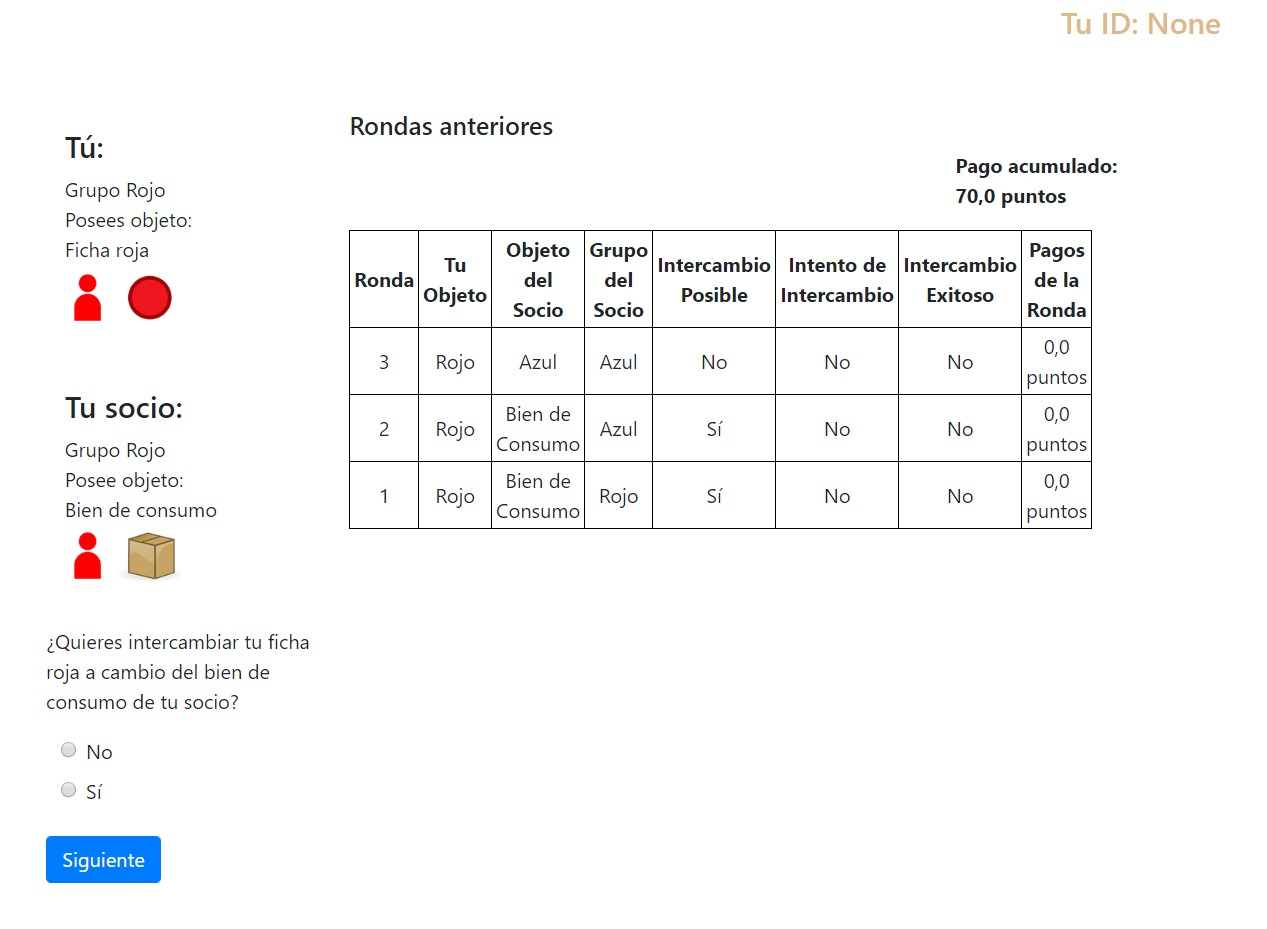
\includegraphics[scale=0.4]{historial2.jpg}
    \caption{Player interface}
    \label{fig:GameScreen}
\end{figure}



\end{document}



